
% this file is called up by thesis.tex
% content in this file will be fed into the main document

%: ----------------------- introduction file header -----------------------
\begin{savequote}[50mm]
The logic of validation allows us to move between the two limits of dogmatism and skepticism. 
\qauthor{Paul Ricoeur}
\end{savequote}


\chapter{Evaluación}
\label{cha:Validation of the methodology}

% the code below specifies where the figures are stored
\ifpdf
    \graphicspath{{5_experiments_and_results/figures/PNG/}{5_experiments_and_results/figures/PDF/}{5_experiments_and_results/figures/}}
\else
    \graphicspath{{5_experiments_and_results/figures/EPS/}{5_experiments_and_results/figures/}}
\fi


%------------------------------------------------------------------------- 

En este capítulo se evalúa la idoneidad del método propuesto para la evaluación de competencias genéricas. Este capítulo se estructura de la siguiente manera:

\begin{itemize}
	\item En primer lugar se describen los entornos de aplicación y las características de los procedimientos que se han utilizado para llevar a cabo la evaluación:
		\begin{itemize}
			\item Publicaciones
			\item Cuestionarios
		\end{itemize}
	\item En segundo lugar se muestran los resultados de la aplicación en cada una de las actividades de aprendizaje para los que se ha implementado el método:
		\begin{itemize}
			\item Wikis: AMW
			\item VLE: SASQL Y EvalCourse
			\item Mundos virtuales: VWQL Y EvalSim
		\end{itemize}
	\item Finalmente se presentan las conclusiones de estas evaluaciones, tanto de los cuestionarios como de las publicaciones.
\end{itemize}

\section{Introducción}

La evaluación del método se ha realizado desde dos perspectivas. Por un lado, cada una de las implementaciones realizadas se ha tratado de mostrar tanto en congresos y revistas de relevancia en el área de las TEL. Mientras que por otro lado, se han realizado cuestionarios y entrevistas a profesionales de la enseñanza para evaluar la idoneidad de los indicadores obtenidos. A continuación se introducen ambos enfoques.

% ---------------------------------------------------------------------
% ---------------------------------------------------------------------
% Inicio entornos de aplicación
% ---------------------------------------------------------------------
% ---------------------------------------------------------------------

% Los entornos de aplicación estaban en el método, pero tras la revisión de Juanma los he movido a este capítulo. Aquí se hablará de ellos, aunque tendré que revisar texto y modificar forma más adelante. Primero abordamos el método.

\subsection{Entornos de aplicación}
\label{sec:tools}

Hay diversos entornos en los que se pueden desarrollar actividades de aprendizaje. Para la implementación del método se seleccionaron tres entornos diferentes: el primer entorno fue un wiki, entorno de trabajo online donde los usuarios crean y editan el contenido de forma colaborativa; el segundo fue un VLE, entorno de aprendizaje virtual donde se alojan cursos virtuales constituidos por una miríada de herramientas; y el tercero un mundo virtual, donde los estudiantes afrontan situaciones de la vida real en un entorno de simulación virtual.

En las próximas secciones se describirán cada una de las herramientas implementadas para aplicar el método en cada uno de los entornos virtuales: AssessMediaWiki para wikis, EvalCourse para VLEs y EvalSim para mundos virtuales.

%------------------------------------------------
\subsubsection{Wikis}

El uso educacional de los wikis para las experiencias de trabajo colaborativo está en auge debido a las numerosas ventajas que aporta sobre los modelos tradicionales~\cite{elgort2008wiki}. Algunas de las ventajas sobre los medios tradicionales, ya sean en formato impreso o en documentos digitales, es que éstos no llevan un registro de ediciones, no permiten la colaboración distribuida y asíncrona y no pueden ser monitorizados por el profesor mientras los estudiantes completan el trabajo.

Para evaluar el trabajo final de un grupo de estudiantes en una página del wiki nos bastaría con leer la última versión de dicha página, como hacíamos con los métodos tradicionales. Pero una de las características más interesantes de los wikis es que no sólo almacenan la información de la versión final de cada documento, sino que también almacenan todas las versiones intermedias creadas como resultado de las contribuciones hechas por cada usuario~\cite{trentin2009using}. Esto lo consigue manteniendo un registro con las diferencias entre las ediciones consecutivas de las páginas, registro que se podría utilizar para la obtención de indicadores de diferentes competencias~\cite{ortega2011new}. Las páginas creadas de manera colaborativa podrían ser evaluadas considerando la contribución de cada autor y las dinámicas de grupo en la creación de la página en tiempo real. Por desgracia, realizar una evaluación detallada de cada contribución realizada en el wiki es imposible de abordar cuando hay muchos usuarios y éstos participan activamente.

En un trabajo anterior se utilizó \emph{StatMediaWiki} (SMW)~\footnote{http://statmediawiki.forja.rediris.es/}, una herramienta que proporciona al profesor información cuantitativa sobre la distribución del trabajo de los estudiantes en las páginas del wiki, es decir, qué parte del trabajo realizado en una página del wiki corresponde a cada estudiante. A partir de esa información cuantitativa se evaluó la distribución del trabajo, el trabajo en equipo y el liderazgo. Sin embargo, el aspecto cualitativo quedó fuera, ya que el experimento sólo consideró el número, el momento y el tamaño de las contribuciones~\cite{palomo2014assessment}.

Para completar el análisis cuantitativo proporcionado por SMW con un análisis cualitativo se desarrolló \emph{AssessMediaWiki} (AMW)~\footnote{http://assessmediawiki.forja.rediris.es}. AMW es una herramienta para realizar una evaluación escalable y cualitativa del trabajo realizado en el wiki mediante procedimientos de autoevaluación, evaluación entre iguales y evaluación del profesor.

\paragraph{AssessMediaWiki (AMW)}

La aplicación creada para poner en práctica este método es AMW. AMW es una aplicación web de código abierto que, al conectarse a una instalación MediaWiki, proporciona procedimientos de autoevaluación, evaluación entre iguales y evaluación del profesor, a la vez que mantiene información sobre esas evaluaciones. AMW pone a disposición de los estudiantes una rúbrica previamente definida por el profesor para que realicen la evaluación (figura\ref{fig:AmwRubrica}). 

\begin{figure}
  \begin{center}
    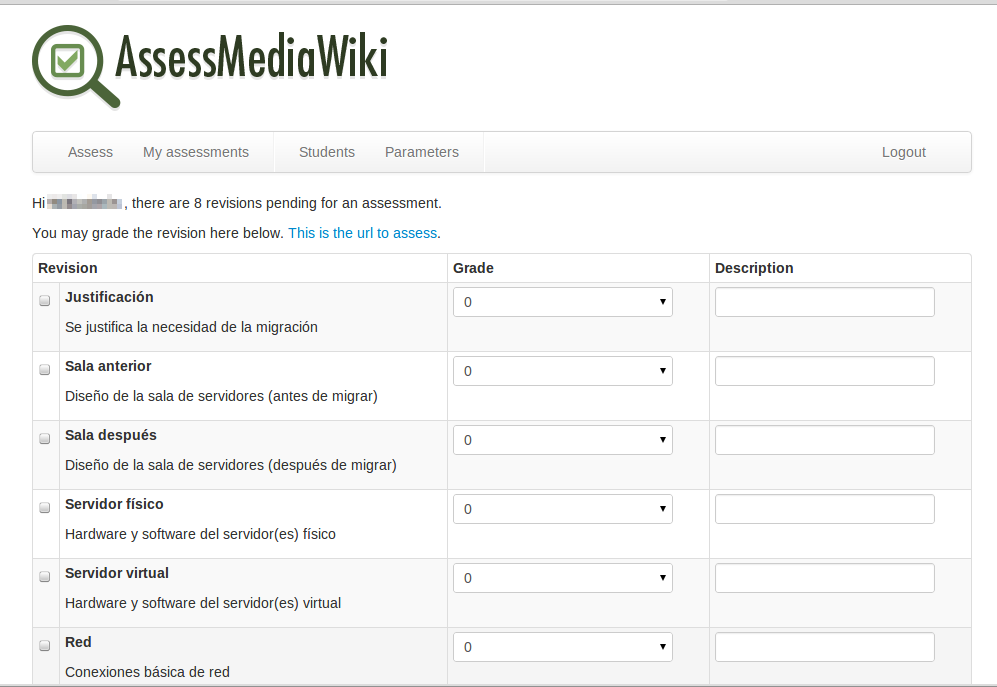
\includegraphics[scale=0.3]{AmwRubrica.png}
  \end{center}
  \caption{Rúbrica de AMW}
  \label{fig:AmwRubrica}
\end{figure}

AMW implementa dos roles de usuario distintos: supervisores y estudiantes. Los estudiantes pueden elegir entre distintas opciones: evaluar una revisión, comprobar sus propias aportaciones evaluadas y verificar las evaluaciones ya enviadas. Por otro lado, los supervisores tienen un mayor número de opciones, como definir la rúbrica que los estudiantes deberán completar al realizar sus evaluaciones, modificar los parámetros de los programas o vigilar las evaluaciones que los alumnos vayan haciendo. AMW implementa un función de selección parcialmente aleatoria. Cuando un estudiante va a realizar una evaluación, el sistema elige automáticamente una de entre el 30\percentage más significativa que aún no ha sido evaluada.

Al revisar sus evaluaciones, los estudiantes puede revisar las notas recibidas y sus justificaciones, así como ver a qué contribución en particular se refiere (figura~\ref{fig:AmwFormative}). Si el estudiante no está de acuerdo con la calificación puede replicar utilizando para ello una réplica similar a la que se utilizó en su evaluación, indicando las calificaciones que considera que merece y sus correspondientes justificaciones. Después el profesor revisará la disputa y pondrá la nota definitiva.

\begin{figure}
  \begin{center}
    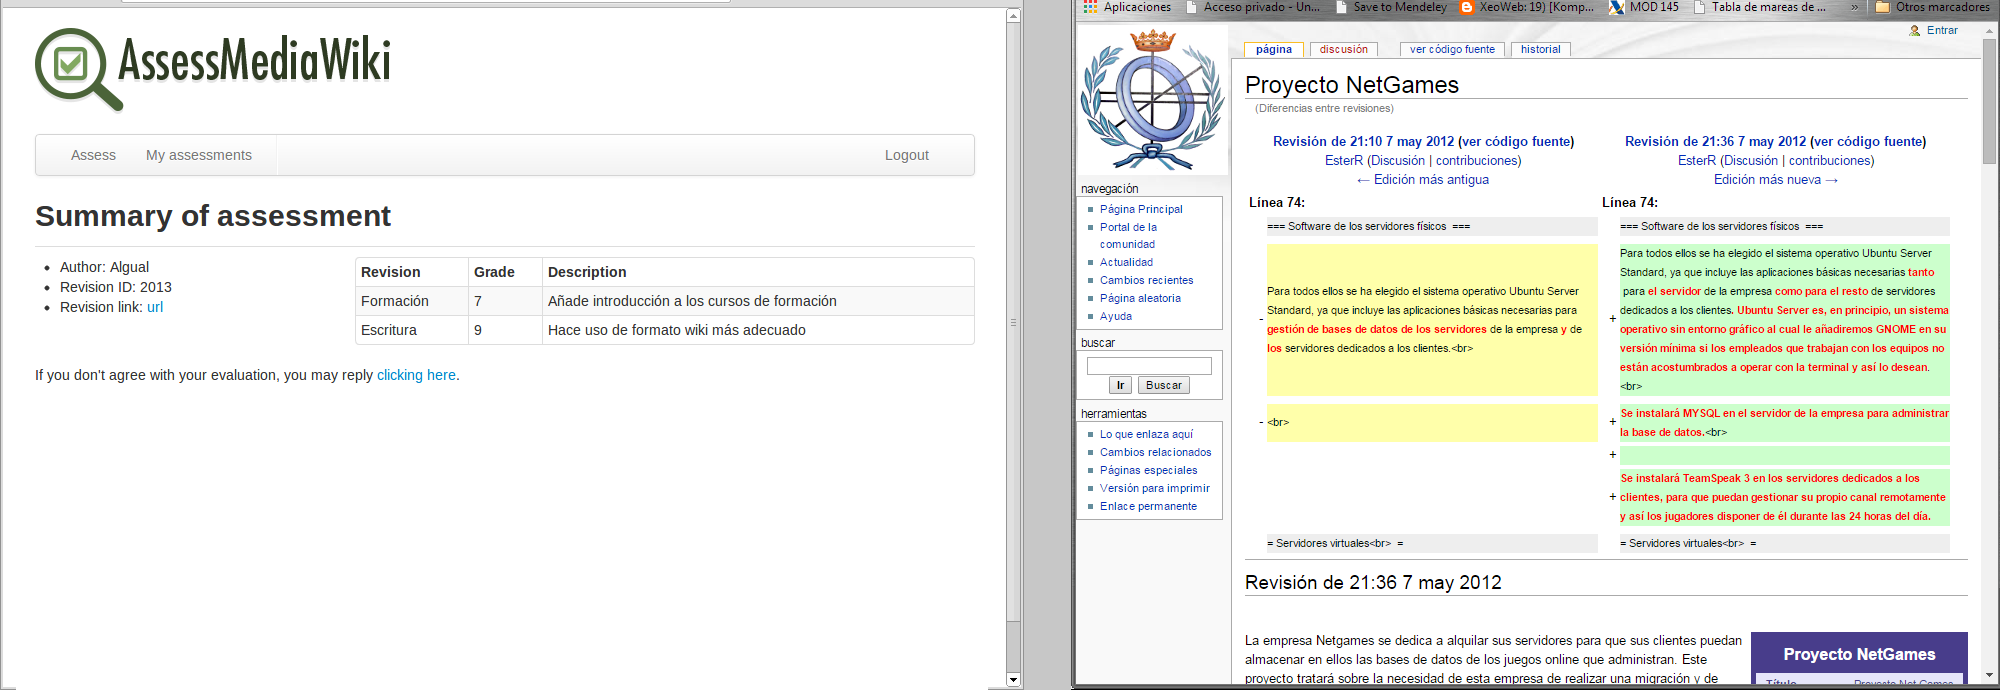
\includegraphics[scale=0.19]{AmwFormative.png}
  \end{center}
  \caption{Ejemplo de retroalimentación formativa y la contribución de wiki evaluada}
  \label{fig:AmwFormative}
\end{figure}

\paragraph{Método}

El método para la evaluación del trabajo y las competencias desempeñadas en el wiki consta de dos partes: una primera parte en la que lo que se evalúa es el trabajo del wiki, basada en procedimientos de autoevaluación, evaluación entre iguales y evaluación del profesor; y una segunda parte en la que se evalúan las competencias genéricas y es donde se pone en práctica el \emph{ciclo de contraste de hipótesis}.

\paragraph{Evaluación del trabajo en el wiki}

El método para la evaluación del trabajo en el wiki se divide también en tres fases: una primera fase en la que los estudiantes realizan sus trabajos en las páginas del wiki, una segunda fase de evaluación y una tercera fase de revisión del profesor. En la figura~\ref{fig:AmwDiagram} puede verse un diagrama de flujo de trabajo que muestra cada una de las fases del método de evaluación realizado sobre una página del wiki en la que participan varios estudiantes y el profesor. A continuación se describen cada una de estas fases.

\begin{figure}
  \begin{center}
    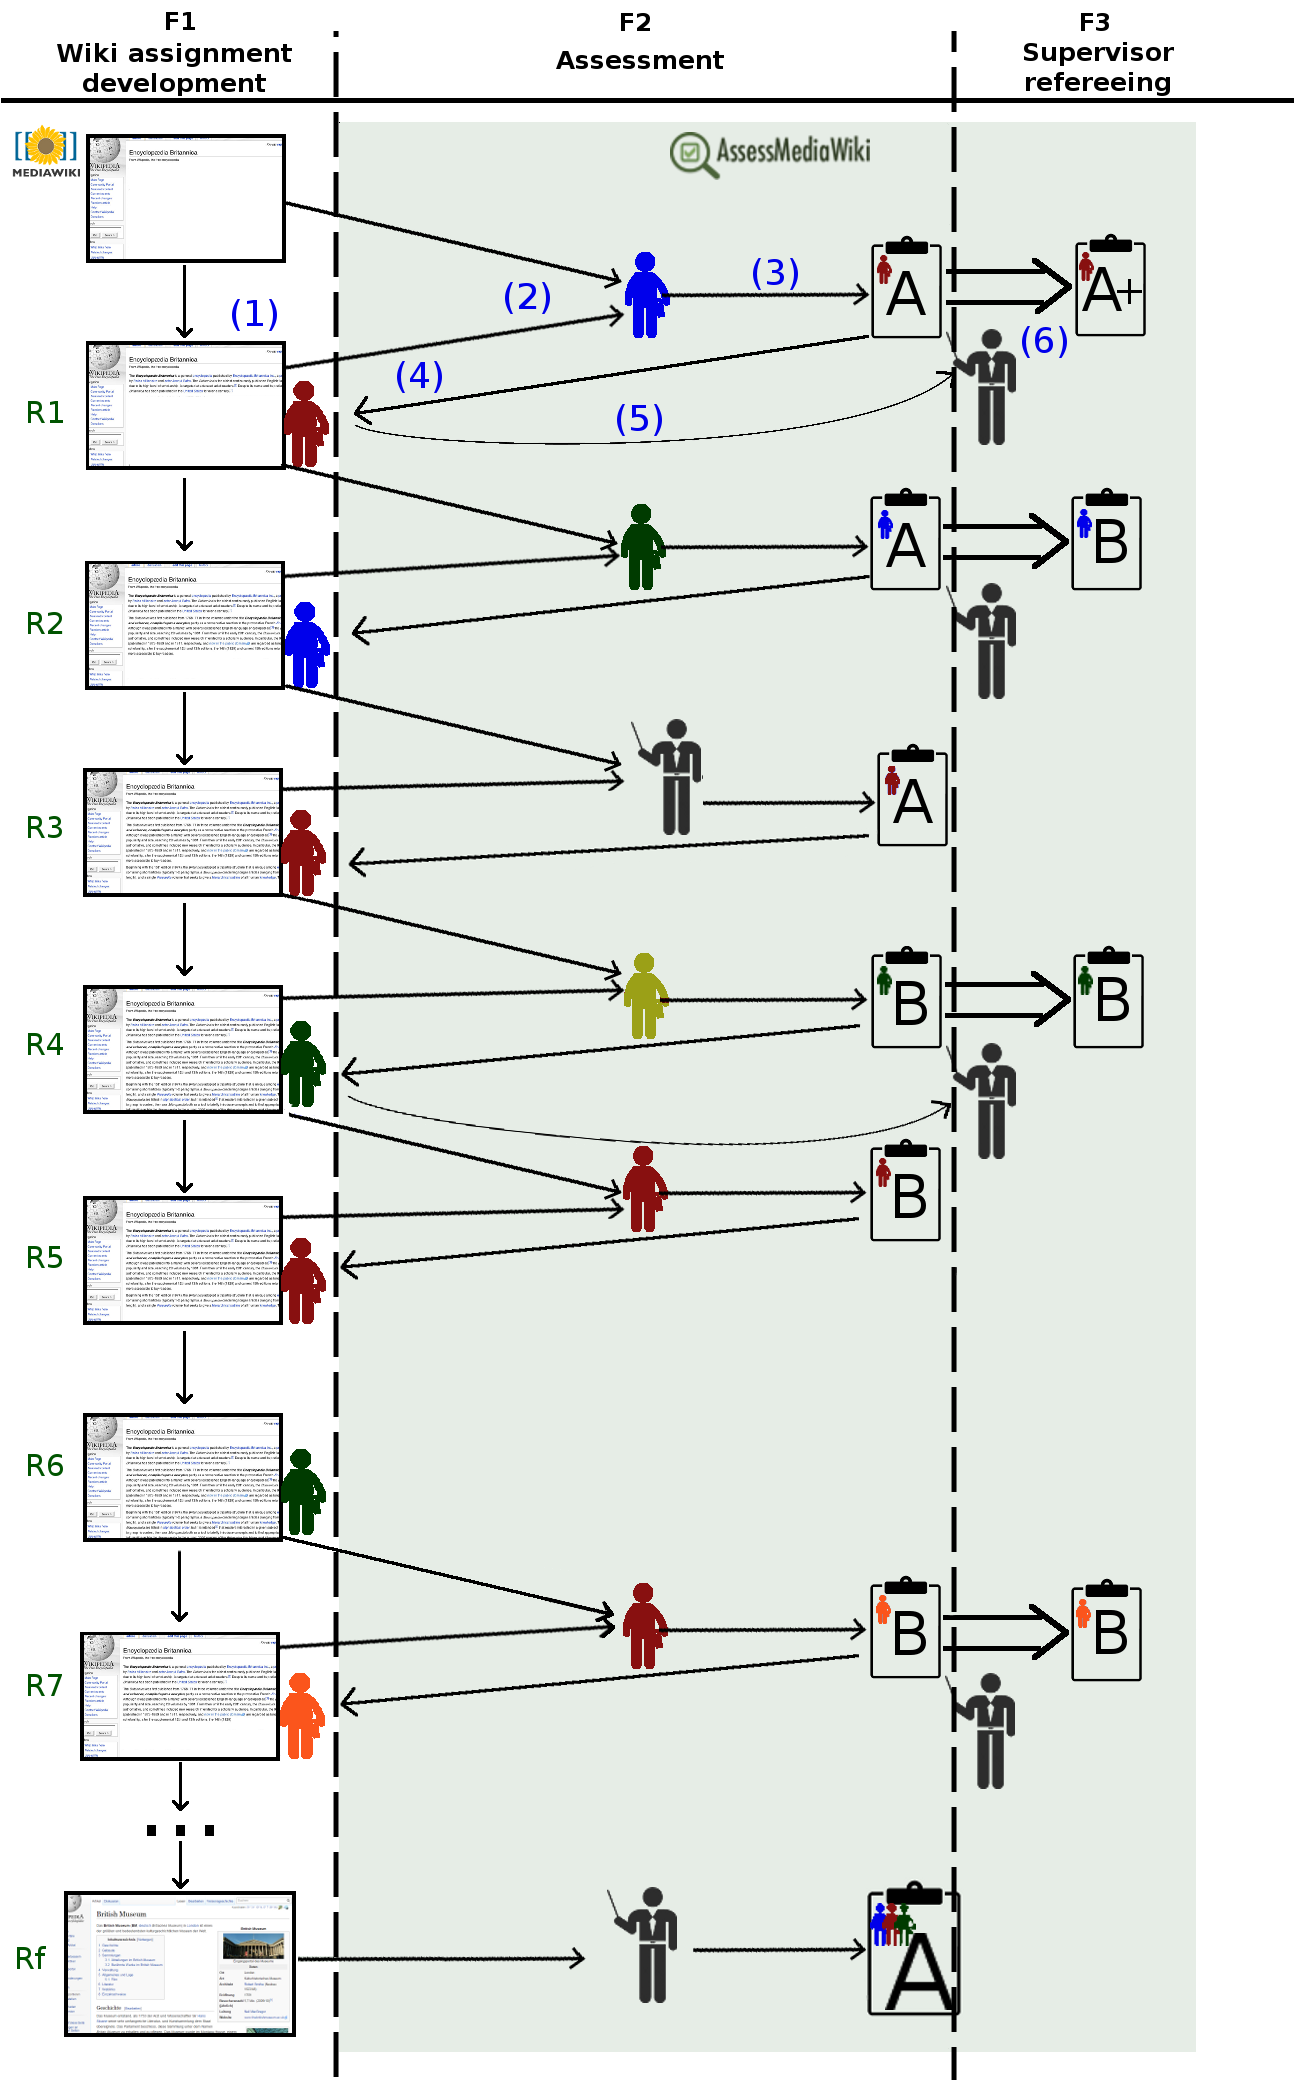
\includegraphics[scale=0.28]{AmwDiagram.png}
  \end{center}
  \caption{Ejemplo de flujo de trabajo para la evaluación cualitativa del wiki utilizando AMW}
  \label{fig:AmwDiagram}
\end{figure}

\paragraph*{Desarrollo del trabajo en el wiki}

Esta fase se representa en la columna de la izquierda de la figura~\ref{fig:AmwDiagram}, y es en la que los estudiantes realizan el trabajo en las páginas del wiki. Normalmente, cada grupo de estudiantes tendrá que desarrollar su trabajos en una página del wiki. En la zona más alta de la columna se representa el comienzo del trabajo con una página en blanco. El autor de cada contribución se muestra con una figura de color junto a la misma. Para comenzar, el usuario de color rojo crea una página vacía (\emph{R1}). Después, el usuario azul añade contenido a la página (\emph{R2}). En tercer lugar, el usuario rojo modifica de nuevo la página añadiendo texto a la versión dejada anteriormente por el usuario azul (\emph{R3}) y así sucesivamente. Esta fase termina cuando llega la fecha marcada por el profesor para que los trabajos estén finalizados (\emph{Rf} es la versión final de la página).

Puede verse que, aunque los estudiantes responsables de la página de ejemplo del wiki fuesen el rojo, el azul y el verde, otros estudiantes, como el naranja en la revisión séptima, podrían contribuir a la página del wiki. En ese caso, los miembros del grupo y responsables de la página deben decidir si la contribución debe conservarse o no.

\paragraph*{Evaluación}

Esta fase se muestra en la columna central y comprende las siguientes actividades:

\begin{itemize}
\item \emph{Autoevaluación, evaluación entre iguales y evaluación del profesor}. Las contribuciones a ser evaluadas se asignan a los estudiantes.  Cada contribución es la diferencia entre dos revisiones consecutivas de una página del wiki. El estudiante encargado de evaluar dicha contribución se representa en el gráfico como un usuario coloreado que recibe dos flechas de las revisiones, una de la revisión anterior a la contribución y otra de la revisión que incorpora ya la contribución. Para la evaluación los estudiantes utilizan una rúbrica definida por el profesor. Cada contribución sólo se refiere a una contribución atómica de las realizadas a una página del wiki por un único estudiante, por lo que dicha contribución podría ser utilizada como un indicador de la contribución al wiki de dicho estudiante. El estudiante que realizó cada contribución se representa con una figura pegada a la revisión de la página en cada momento.
Por ejemplo, en la primera evaluación, se asigna la contribución realizada a la página del wiki por el estudiante rojo (\emph{1}) al estudiante azul. El estudiante azul comprueba ambas versiones para ver las diferencias entre ambas versiones (\emph{2}) y realiza la evaluación completando la rúbrica proporcionada por el profesor (\emph{3}).
Cabe destacar también otras situaciones interesante. En la versión \emph{R5} de la página vemos como se realiza una autoevaluación, ya que el estudiante rojo, autor de la versión, es el mismo que tiene que evaluar su contribución. Vemos también que en \emph{R3} es el profesor el que realiza la evaluación de la contribución del estudiante rojo. Esto puede deberse a que el estudiante manualmente detecta una contribución que considera oportuno evaluar o a que, utilizando la herramienta SMW, detecta un comportamiento extraño en el wiki y quiere contrastar la situación. 
Puede verse también que hay contribuciones que no reciben evaluación alguna, como ocurre con \emph{R6}. Está claro que sería deseable que todas las contribuciones significativas fueran evaluadas, pero no es escalable.
\item \emph{Revisión de las evaluaciones recibidas}. Los estudiantes pueden revisar las evaluaciones recibidas. Ellos pueden no sólo ver las notas que han recibido con las justificaciones y comentarios que añadieron sus evaluadores, sino también el enlace a la contribución. De esta forma, los estudiantes evaluados reciben una retroalimentación formativa. En la primera de las evaluaciones del diagrama de ejemplo puede verse como el estudiante rojo puede ver su evaluación (\emph{4}).
\item \emph{Réplica}. Si el estudiante evaluado no está de acuerdo con la evaluación recibida tiene la opción de replicarla justificando el motivo de dicha réplica. En el diagrama de ejemplo puede verse como el estudiante rojo considera injusta su evaluación y realiza una réplica (\emph{5}). El profesor deberá resolver la réplica en la siguiente etapa.
\item \emph{Evaluación final del wiki}. El profesor evalúa la versión final de la página del wiki desarrollada por cada grupo de estudiantes. Esta evaluación es necesaria ya que el objetivo principal de la tarea es que los estudiantes realicen un buen trabajo en una página del wiki. Como cualquier otra tarea, deberá ser evaluada por el profesor conforme al programa de estudios. Además, algunos de los criterios de evaluación sólo pueden ser evaluados en la versión final de la página, como por ejemplo, la coherencia del texto. De esta forma, aquellas contribuciones del wiki descartadas por la función de selección serán ahora implícitamente evaluadas ya que están integradas en el entregable final. Puede verse la evaluación al final del diagrama de ejemplo (\emph{Rf}), y cómo afecta al grupo de estudiantes completo.
\end{itemize}

El diagrama no recoge algunas situaciones que también podrían darse. Por ejemplo, alguna contribución podría ser evaluada por más de un usuario, ya fuera otro estudiante o el profesor. También, para simplificar, el diagrama sólo muestra una calificación para la contribución (A, A+, B, ... etc.), pero las evaluaciones son multidimensionales.

Un componente interesante de nuestro algoritmo es qué contribución wiki podrá ser asignada a cada estudiante para su evaluación. Es lo que llamamos \emph{función de selección}, y tiene varios aspectos a tener en cuenta:

\begin{itemize}
\item \emph{¿Debería cierta contribución en el wiki ser evaluada por más de un estudiante?} En realidad, tener varias evaluaciones de estudiantes diferentes sobre una misma contribución podría ser interesante para perfeccionar su evaluación y podría proporcionar información al profesor para evaluar no sólo al estudiante autor de la contribución, sino también a los evaluadores. De hecho, el número de contribuciones a ser evaluadas es dependiente del objetivo del experimento y su configuración. Cuánto más grande sea el experimento, más contribuciones susceptibles de ser evaluadas tendrá. Sin embargo, el número de evaluaciones que un estudiante puede realizar es limitado (para que siga siendo formativo). Por lo que cada evaluación adicional a la misma contribución provocará que otras contribuciones sean más pobremente evaluadas o que no lo sean.
\item \emph{¿Qué contribuciones deberían ser evaluadas?} La importancia de evaluar cada contribución puede variar. Por ejemplo, evaluar al menos una mínima cantidad de contribuciones por cada estudiante, página o categoría sería interesante. Pero algunas contribuciones que añadan ciertas características al trabajo pueden ser relevantes o informativas sobre el trabajo realizado por un estudiante. Por ejemplo, aunque las contribuciones que añadan gran cantidad de texto suelan ser más interesantes que las contribuciones pequeñas, una contribución pequeña puede ir relacionada con el cambio de sentido de alguna frase o párrafo. De cualquier forma, un estudiante puede solicitar que una contribución en particular sea evaluada, aunque ésta quede fuera de la función de selección.
\item \emph{¿Quién evalúa cada contribución?} Depende de la importancia que se quiera dar a la autoevaluación, la evaluación del compañero y la del profesor. De nuevo, se debería balancear el esfuerzo requerido y el detalle a exigir en las evaluaciones.
\end{itemize}


\paragraph*{Revisión del profesor}

En esta última columna se representan dos actividades que corresponden al profesor:

\begin{itemize}
\item Resolución de las réplicas: el profesor revisa las réplicas indicando si proceden o no. En caso de que procedan, modifica la calificación. En el diagrama se puede ver como en la primera contribución, el estudiante rojo realiza una réplica (\emph{5}) sobre la evaluación reciba por el usuario azul (\emph{3}). El profesor revisa la réplica, la considera apropiada y modifica la calificación (\emph{6}). En un segundo ejemplo, en la evaluación realizada por el estudiante de color amarillo sobre la contribución realizada por el usuario de color verde puede verse como el profesor no acepta la réplica realizada por este último, y mantiene la calificación otorgada inicialmente por el estudiante amarillo.
\item Revisión de evaluaciones no replicadas: el profesor puede revisar aleatoriamente otras evaluaciones realizadas por los estudiantes que no hayan sido replicadas. En el diagrama puede verse como en el profesor revisa las evaluaciones realizadas sobre las contribuciones representadas en \emph{R2} y en \emph{R7}, disminuyendo la calificación de la primera y manteniendo la segunda.
\end{itemize}

\paragraph{Evaluación de competencias genéricas}

El método para la evaluación de competencias genéricas se basa en el \emph{ciclo de contraste de hipótesis}. En la figura~\ref{fig:AmwDiagram2} puede verse la descripción del método. Esta evaluación se puede llevar a cabo durante o después de que los estudiantes hayan realizado su trabajo en el wiki y sus evaluaciones con AMW. Evidentemente, cuánto más avanzado esté el trabajo más datos habrá para analizar. 

El ciclo comienza con el diseño de un indicador por parte del profesor que plasmará en una hoja de cálculo a partir de los datos que recibirá de las evaluaciones (a). A continuación, el profesor realiza la petición a AMW que le proporcionará los datos (b). AMW consulta y procesa los datos en las bases de datos de MediaWiki y AMW (c) y se los envía al profesor (d). El profesor los integra en la hoja de cálculo previamente diseñada y los analiza (e). Si son válidos para la evaluación finaliza el proceso (f). Por el contrario, si necesitan algún tipo de refinamiento el profesor puede rediseñar la evaluación (g) y hacer una nueva petición.

\begin{figure}
  \begin{center}
    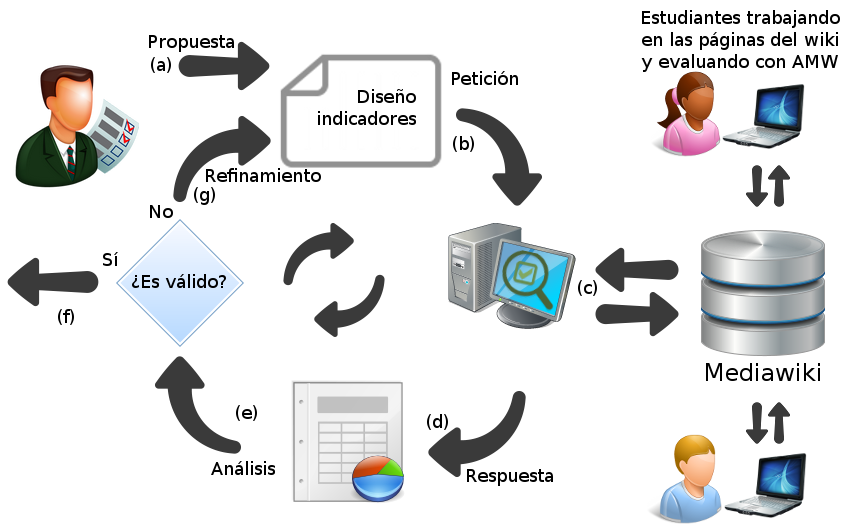
\includegraphics[scale=0.45]{AmwDiagram2.png}
  \end{center}
  \caption{Ciclo de contraste de hipótesis para la evaluación en wikis}
  \label{fig:AmwDiagram2}
\end{figure}

\paragraph{Indicadores}

Los indicadores que se mencionan en este punto han sido utilizados en los estudios de caso realizados para este trabajo, pero como se ha mencionado desde un primer momento, este método proporciona indicadores y es el profesor el que los utilizará para evaluar las competencias genéricas que considere oportunas.

\paragraph*{Trabajo en equipo}
El indicador considerado para el trabajo en equipo es el \emph{ratio de miembros del equipo que trabajaron en un mismo criterio.} La rúbrica que utilizan los estudiantes para evaluar se compone de un conjunto de criterios. Cada criterio puede hacer referencia a una parte del trabajo. En todas las ediciones de un wiki no se trabajan en las mismas partes del trabajo, por lo que al ser evaluado, un estudiante puede tener nota en unos criterios y no tenerla en otros. Si más de un estudiante ha trabajado en la misma parte de una página wiki y su aportación ha sido significativa, tendrán nota en dicho criterio. Por tanto, partiendo de la cantidad de criterios que tiene un trabajo y del ratio de miembros del equipo que ha trabajado en cada criterio tendremos un indicador del trabajo en equipo.

\paragraph*{Comunicación y aplicación del conocimiento}
El indicador considerado para la comunicación y la aplicación del conocimiento es la \emph{media de las notas recibidas por todos los miembros del grupo}. Este indicador mide la incidencia que tuvieron las contribuciones realizadas en el éxito del proyecto. Una calificación pobre en una contribución puede significar  que alguna contribución wiki obtuvo una buena nota en un cierto criterio de la rúbrica pero una mala nota en el otro (el autor de la contribución soluciona un problema y crea uno nuevo). Probablemente, esto se debió a una mala comunicación entre los miembros del equipo o poco compromiso de un determinado alumno en el objetivo global del grupo. 

\paragraph*{Mantener la calidad del trabajo producido}
El indicador considerado para el mantenimiento de la calidad del trabajo producido es la \emph{media de las notas que cada estudiante individualmente recibió}. Unas calificaciones altas en las evaluaciones recibidas pueden significar que el trabajo que el estudiante está produciendo es de calidad. Si el estudiante produjese mucho contenido, pero este no fuese de calidad, las calificaciones no serían buenas. Es decir, sus calificaciones están teniendo en cuenta el aspecto cualitativo del trabajo y por tanto una nota alta significaría un trabajo de calidad.

\paragraph*{Capacidad crítica}
El indicador considerado para la capacidad crítica es el \emph{número de evaluaciones que el estudiante realizó con respecto al número de dichas evaluaciones cuya nota fue modificada por el profesor}. Este indicador mide la competencia de un estudiante para evaluar el trabajo hecho por otros. Si recibiera un número fijado de réplicas en sus revisiones y estas fueran revisadas por el profesor modificando las calificaciones, podríamos considerar que dicho alumno no ha desempeñado bien dicha competencia.

En la tabla~\ref{tab:ResumenIndicadoresCualiCuanti} puede verse una comparación entre los indicadores considerados a partir de la evaluación cualitativa que se realizaría con AMW y los que se obtienen a partir de la evaluación cuantitativa realizada con SMW.

\begin{table}
  \begin{center}
  \begin{tabular}{| m{3.2cm} | m{4.9cm} | m{5.1cm} |}
    \hline 
    \multirow{2}{*}{COMPETENCIAS}  & INDICADORES  & INDICADORES  \\
      &  CUALITATIVOS  &  CUANTITATIVOS \\
    \hline
    \hline
    Trabajo en equipo  & Ratio de miembros del equipo que trabajaron en un mismo criterio  & Ratio de miembros del equipo que contribuyeron a una misma página del wiki en las páginas de su proyecto \\
    \hline
    Comunicación y aplicación del conocimiento  & Media de las notas recibidas por todos los miembros del grupo  & Porcentaje de miembros del equipo que contribuyeron al menos a un 20\percentage del trabajo realizado \\
    \hline
    Mantener la calidad del trabajo producido  & Media de las notas que cada estudiante individualmente recibió  & Contribución individual en bytes \\
    \hline
    Capacidad crítica  & Número de evaluaciones que el estudiante realizó con respecto al número de dichas evaluaciones cuya nota fue modificada por el profesor  & No considerada \\
    \hline
  \end{tabular}
\end{center}
\caption{Resumen de las competencias evaluadas para cada tipo de indicador}
\label{tab:ResumenIndicadoresCualiCuanti}
\end{table} 

%\subsubsection{Ejemplo de uso}

%El ejemplo de uso podrá verse en el estudio de caso que se muestra en el siguiente capítulo.
%\subsubsection{Publicación}

%Un trabajo con AMW fue publicado en SPDECE 2012~\cite{Balderas:2012}.
% La evaluación de las 3 herramientas se corresponde al capítulo siguiente.

%-----------------------------------------------------------------------------------------------------------------------------------------------
\subsubsection{VLE}

En esta segunda propuesta el método se aplica a los cursos virtuales. El VLE es el núcleo de los cursos virtuales, donde los profesores ponen el material a disposición de los estudiantes y donde los estudiantes pueden fácilmente acceder a ellos; donde tanto los profesores como los estudiantes se pueden comunicar entre ellos de manera síncrona y asíncrona; y donde los estudiantes gestionan sus proyectos en equipo mientras dialogan entre ellos. Gracias a la gran cantidad de información que genera la actividad de los estudiantes y que queda registrada en el VLE, los investigadores de diferentes áreas han colaborado para extraerlos, realizar minería de datos y utilizarlos para mejorar el aprendizaje~\cite{park2015development}.

Además, en algunos de los trabajo recopilados en el estado del arte mostrado en el capítulo~\ref{cha:State of the Art}, se confirma la relación entre la interacción que llevan a cabo los estudiantes en el VLE y su rendimiento en el desempeño de varias competencias genéricas~\cite{fidalgo:2015,rayon2014web}. 

Por tanto, y tal y cómo se mostrará a continuación, en esta propuesta se utilizarán indicadores obtenidos de la interacción de los estudiantes en el VLE para el diseño de evaluaciones de competencias genéricas dentro del  \emph{ciclo de contraste de hipótesis}.


\paragraph{SASQL y EvalCourse}

Para diseñar evaluaciones a partir de los indicadores del VLE se crea un lenguaje especifico de dominio (DSL, del inglés \emph{domain-specific language})~\cite{vanDeursen:2000}: \emph{Simple Assessment-Specific Query Language} (SASQL). Es un lenguaje formal para la ejecución automática de consultas simples escritas utilizando un lenguaje específico de evaluación. SASQL tiene un sintaxis simple, orientada a la evaluación de competencias genéricas~\cite{Balderas:2013}. De esta forma, los profesores pueden fácilmente obtener indicadores almacenados de la actividad en el VLE sin requerir conocimientos técnicos en bases de datos o programación informática.

También se implementa \emph{EvalCourse}, una herramienta informática que ejecuta instrucciones escritas en SASQL, proporcionando como resultado los indicadores solicitados. EvalCourse se comunica con el VLE para extraer la información del registro de actividad. EvalCourse\footnote{https://www.assembla.com/spaces/evalcourse} está basado en el IDE de la plataforma Eclipse, fue implementado utilizando Xtext~\cite{eysholdt2010xtext} dentro del Eclipse Modeling Framework y está disponible como software libre bajo licencia GNU GPL.

El desarrollo de EvalCourse y SASQL se basa en los principios y técnicas de la ingeniería dirigida por modelos (MDE, del inglés Model-Driven Engineering). Este enfoque promueve la construcción de artefactos software de un modo flexible y rápido mediante el desarrollo de modelos y sus transformaciones. Nuestro DSL se define en términos de su sintaxis abstracta o metamodelo, su sintaxis concreta y un conjunto de plantillas para la transformación de modelos de consulta en código ejecutable dependiente del VLE.

\begin{figure}
  \begin{center}
    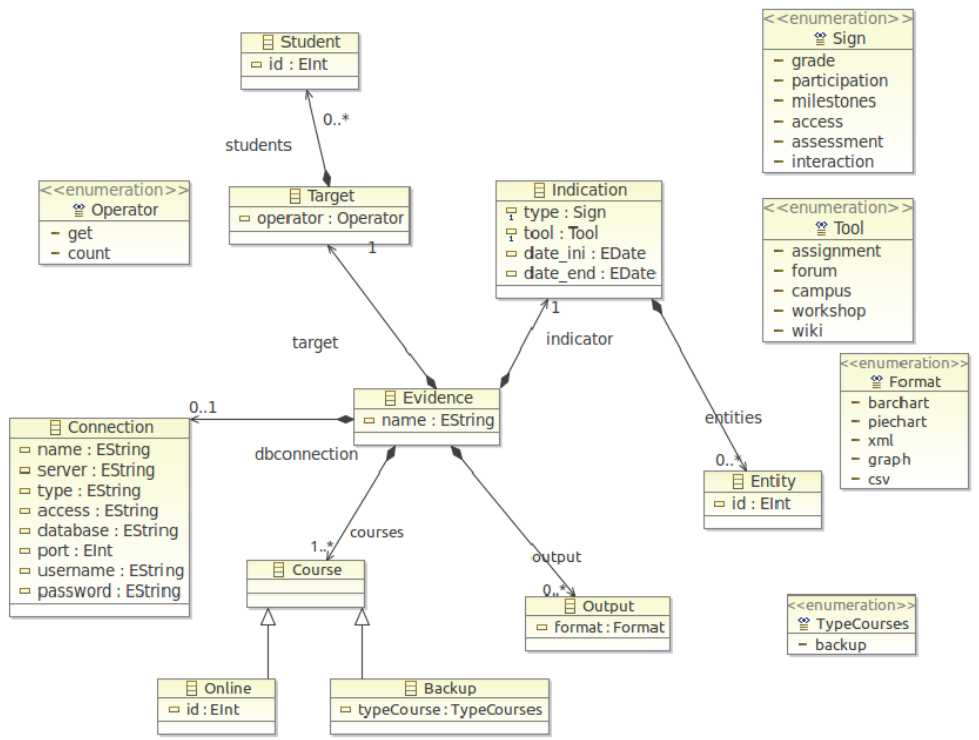
\includegraphics[scale=0.4]{EvcMetamodel.png}
  \end{center}
  \caption{Metamodelo de SASQL}
  \label{fig:EvcMetamodel}
\end{figure}

El metamodelo de EvalCourse puede verse en la figura~\ref{fig:EvcMetamodel}. La entidad principal es el indicador o evidencia (\emph{evidence}). Esta evidencia se aplicará a una herramienta (\emph{tool}) que puede ser tarea (\emph{assignment}), foro (\emph{forum}), campus (\emph{campus}), taller (\emph{workshop}) o wiki (\emph{wiki}), en las que se observará un indicio (\emph{sign}), que puede ser participación (\emph{participation}), entregas (\emph{milestones}), accesos (\emph{access}), evaluaciones (\emph{assessment}), interacción (\emph{interaction}) o calificación (\emph{grade}). Además, puede actuarse sobre una actividad específica (\emph{entity}) o sobre todas las actividades de un tipo que se han dado en el VLE. La conexión a la base de datos del curso se declara en la entidad \emph{connection}. 

La sintaxis de SASQL puede verse en la consulta~\ref{code:sasqlSintax}. En la primera línea se comienza con la palabra reservada \emph{Evidence} seguida del nombre que se dará al indicador. Ese nombre será el que tengan todos los ficheros de salida. En la segunda línea se escriben los términos obligatorios \emph{get students}. En la tercera, se indica qué indicio se quiere extraer (\emph{show milestones | participation | access | interaction | assessment | grade}). En la consulta, la tercera línea se divide en dos (tercera y cuarta) para que puedan ser visualizadas todas las opciones. En la quinta, se indica sobre qué herramienta se quiere obtener el indicio (\emph{ in assignment | forum | campus | workshop | wiki [list of ids]}). También la quinta línea se divide en dos (quinta y sexta). En la séptima línea, que es opcional, se indica el rango de fechas sobre los que se extraerá la información. Y por último, en la octava se especifica si la conexión se realizará directamente a la base de datos o sobre una copia de seguridad almacenada en un fichero.

\begin{lstlisting}[caption=Sintaxis de SASQL (las palabras reservadas se muestran resaltadas),label=code:sasqlSintax,numbers=left, captionpos=b, morekeywords={Evidence,get, students, show, milestones, participation, access, in, assignment, forum, campus, wiki, between, and, workshop, interaction, assessment, grade, from, course, backup}]
Evidence indicator_name:
 get students 
 show milestones | participation | access 
	| interaction | assessment | grade
 in assignment | forum | campus | workshop 
	| wiki [list of ids]
 between YYYY-MM-DD and YYYY-MM-DD
 from course id | backup.
\end{lstlisting}

El objetivo es que EvalCourse pueda ser utilizado para cualquier VLE, pero esta primera versión ha sido implementada para funcionar en Moodle~\footnote{https://moodle.org/}. Moodle es un sistema de gestión de aprendizaje de código abierto con más de 64.000 sitios registrados~\footnote{https://moodle.net/stats}, y que además es el que se utiliza en la Universidad de Cádiz.

\paragraph{Método}

Para evaluar las competencias genéricas el profesor deberá definir los indicadores que serán extraídos de la actividad de cada estudiante en el VLE. Ilustraremos el método a partir de un ejemplo de uso de EvalCourse y su ejecución con los foros del VLE. Los foros suelen ser una de las herramientas incorporadas por los VLEs para la interacción entre los estudiantes. Es evidente que la comunicación oral es una manera muy rica de comunicarse, que proporciona múltiples signos no verbales como las expresiones faciales o el tono de voz. En contraste, las comunicaciones escritas proporcionan otras ventajas. Una de las más importantes para la educación es que el estudiante dispone de un tiempo para la reflexión. Por esta razón, podría preferirse la comunicación escrita a la oral cuando se busca un aprendizaje cognitivo~\cite{garrison1999critical}.

La obtención de indicadores se basará en el \emph{ciclo de contraste de hipótesis}(figura~\ref{fig:EVCDiagram}). En primer lugar, es necesario que los estudiantes hayan interactuado en el VLE, de manera que su actividad haya quedado registrada. Entonces, el profesor propone un diseño de evaluación mediante una consulta SASQL (a) y envía esta consulta a EvalCourse (b). EvalCourse procesa la consulta, realiza la petición a la base de datos y recoge los datos (c). Entonces EvalCourse devuelve los resultados (d). El profesor analiza los resultados conforme a su propuesta de evaluación de competencias (e), terminando el proceso si éstos son válidos para él (f). Por el contrario, si los resultados no son válidos como indicadores de la competencia, entonces el profesor podrá rediseñar la evaluación (g). En cualquier caso, el profesor podrá reutilizar el diseño cuántas veces sea necesaria a lo largo del curso y monitorizar la evolución de los indicadores de cada estudiante.

\begin{figure}
  \begin{center}
    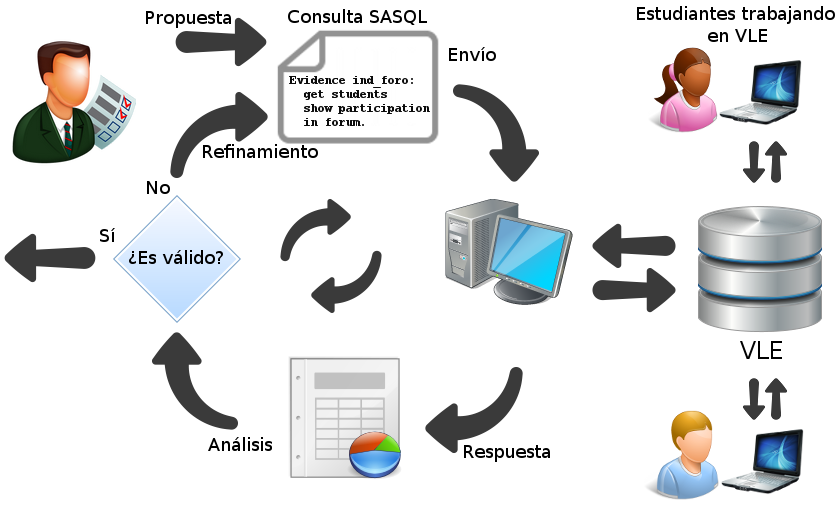
\includegraphics[scale=0.45]{EvcDiagram.png}
  \end{center}
  \caption{Ciclo de contraste de hipótesis utilizando EvalCourse}
  \label{fig:EVCDiagram}
\end{figure}

\paragraph*{Ejemplo de uso}

En este ejemplo, el profesor pretende obtener indicadores del uso del foro para evaluar la competencia genérica de las habilidades interpersonales. Durante el curso, los estudiantes interactuarán en el foro conforme a las instrucciones proporcionadas por el profesor. Cuando lo desee, el profesor podrá utilizar EvalCourse para obtener los indicadores.

% Estos indicadores deben ser publicados para que los estudiantes sepan cómo serán evaluados % FRASE ELIMINADA DEL MEDIO DEL PÁRRAFO ANTERIOR

El profesor considera que podría diseñar un indicador válido a partir del número de mensajes que ha escrito cada estudiante en un periodo de tiempo particular y plantea la siguiente hipótesis: \emph{se considerará que un estudiante ha desempeñado satisfactoriamente la competencia genérica de las habilidades interpersonales si ha escrito al menos dos mensajes en el foro}. Para ello se diseña la consulta~\ref{code:sasqlejemplo1}. EvalCourse procesa la consulta y devuelve los resultados que se pueden ver en la tabla~\ref{tab:EvalCourseEj1}.

\begin{lstlisting}[caption=Participación en el foro en un periodo concreto de tiempo ,label=code:sasqlejemplo1,numbers=left, captionpos=b, morekeywords={Evidence,get, students, show, milestones, participation, access, in, assignment, forum, campus, workshop, interaction, between, and}]
Evidence participacion_foro: 
	get students
	show participation
	in forum between 2015-10-21 and 2015-10-27.
\end{lstlisting}

\begin{table}
	\centering
	\caption{Información sobre la participación en el foro de los estudiantes en un periodo concreto de tiempo}
	\label{tab:EvalCourseEj1}
	\begin{tabular}{|l|l|c|c|c|c|c|}
		\hline
		id & username & Debate-starter & Debate-participation & Total \\
		\hline
		\hline
		1 & student1 & 1 & 2 & 3  \\
		\hline
		2 & student2 & 0 & 4 & 4  \\
		\hline
		3 & student3 & 0 & 1 & 1  \\
		\hline
		4 & student4 & 1 & 2 & 3  \\
		\hline
		5 & student5 & 0 & 2 & 2  \\
		\hline
	\end{tabular}
\end{table}

A la vista de los resultados, y en base a la hipótesis inicial, se podría decir que todos los estudiantes menos el 3 (\emph{student3}) habrían desempeñado correctamente la competencia. Sin embargo, el profesor considera que esta primera aproximación es un poco pobre y decide completar su hipótesis de la siguiente manera: \emph{se considerará que un estudiante ha desempeñado satisfactoriamente la competencia genérica de las habilidades interpersonales si ha escrito al menos dos mensajes en el foro y ha interactuado con más de un compañero}. Para ello escribe la consulta~\ref{code:sasqlejemplo2}. 

\begin{lstlisting}[caption=Interacción en el foro en un periodo de tiempo ,label=code:sasqlejemplo2,numbers=left, captionpos=b, morekeywords={Evidence,get, students, show, milestones, participation, access, in, assignment, forum, campus, workshop, interaction, between, and}]
Evidence interacciones_foro: 
	get students
	show interaction
	in forum between 2013-10-21 and 2013-10-27.
\end{lstlisting}

Además del listado con las interacciones, EvalCourse proporciona varias figuras con la representación de la información. Para esta última consulta se devuelve un grafo para una mejor visualización de las interacciones (figura~\ref{fig:EvalCourseInteraccionForo}). A tenor de los resultados vemos que sólo dos de los estudiantes cumplen la segunda hipótesis (\emph{student2} y \emph{student4}). 

\begin{figure}
	\centering
	\includegraphics[width=6cm]{{EvalCourseInteraccionForo.png}}
	\caption{Interacción en el foro en un periodo de tiempo.}
	\label{fig:EvalCourseInteraccionForo}
\end{figure}

De esta manera, el profesor irá redefiniendo sus hipótesis hasta dar con los indicadores que a su juicio satisfagan la evaluación de la competencia genérica.

\paragraph{Indicadores}

En este apartado se muestra una propuesta de uso de indicadores obtenidos mediante EvalCourse para la evaluación de competencias genéricas~\cite{Balderas:2015}. Pero al igual que ocurre con el resto de herramientas, estos indicadores podrían ser válidos para unos profesores y no serlos para otros, así como que habrá otras muchas formas de combinar la información del registro para obtener indicadores válidos para otras competencias genéricas.

\paragraph*{Habilidades interpersonales}
Para la evaluación de esta competencia genérica se propone utilizar la participación en el foro. Al crear grupos de trabajo en el VLE se puede crear un foro para cada grupo. Durante el curso se fomenta que los estudiantes intervengan en dichos foros para comunicarse entre los miembros del equipo y dejar constancia de los mensajes de cara al profesor. Por tanto, si no utilizan el foro, los estudiantes no tienen calificación en esta competencia. Por ejemplo, podría fijarse que un estudiante que tuviera tres o más intervenciones en el foro tendría una evaluación positiva en la competencia.

\paragraph*{Liderazgo}
Para evaluar el liderazgo de los estudiantes se proponen también los foros creados para la comunicación de los equipos de trabajo. Para ello se podría considerar la cantidad de debates que cada estudiante ha iniciado. Por ejemplo, un estudiante que iniciara dos o más debates tendría una evaluación positiva en la competencia de liderazgo.

\paragraph*{Pensamiento crítico}
En Moodle hay una actividad que son los talleres (\emph{workshops}). En esta actividad, los estudiantes tienen que entregar un ejercicio conforme a las instrucciones del profesor que podrá ser autoevaluada o evaluada por uno o varios compañeros. Por ejemplo, podría plantearse que cada estudiante tuviera que hacer varias tareas. Una vez entregada cada tarea, el profesor pondría la solución del ejercicio a disposición de los estudiantes, y cada tarea sería evaluada por dos compañeros y por el propio estudiante. Para evaluar la competencia del pensamiento crítico, el profesor utilizaría para cada tarea la diferencia entre la media de las notas dadas por sus compañeros y la que se asignó el propio estudiante.

\paragraph*{Planificación y gestión del tiempo}
Las tareas programadas en el VLE tienen una fecha límite de entrega. Sin embargo, el profesor puede configurar la actividad para que permita envíos retrasados. El profesor podría establecer un número mínimo de trabajos entregados antes de la fecha límite para considerar que esta se ha entregado a tiempo. De esta manera, un profesor podría considerar que si las tareas se han entregado tarde, pero son correctas, tengan una buena calificación en lo que a las habilidades y conocimientos específicos que requería la tarea se refiere. Pero con respecto a la planificación y gestión del tiempo de ese estudiante la calificación sería negativa, dado que ha incumplido la planificación y los plazos que se acordaron a comienzos del curso.

%------------------------------------------------------------------------------------------------------------------------------------------------
\subsubsection{Mundos virtuales}

Aunque muchos investigadores han reconocido la potencia educativa y motivacional de los videojuegos, hay pocos estudios empíricos que hayan investigado recientemente su impacto en el aprendizaje de los estudiantes~\cite{berns2013game}. Lo mismo se puede decir de los entornos de aprendizaje como los mundos virtuales (Second Life, OpenCobalt, etc.)~\cite{hew2010use}. Esto se debe a que normalmente no se distribuyen bajo licencia libre y, por consiguiente, los profesores no pueden analizar las interacciones de los estudiantes o analizar su impacto en el aprendizaje y en los resultados de aprendizaje~\cite{cruz2015discovering,moreno2014serious}. 

Ante esta situación, en un trabajo previo desarrollamos nuestro propio mundo virtual, basado en OpenSim (software de código abierto)~\cite{berns2013using}. De esta forma se podría evaluar la competencia de la comunicación en una segunda lengua a partir de las interacciones llevadas a cabo por los estudiantes en el mundo virtual . 

A continuación se explicará cómo a partir de la actividad generada por los estudiantes se obtendrán indicadores para el diseño de evaluaciones de competencias genéricas.

\paragraph{VWQL y EvalSim}

% Habrá que citar antes el MDD {schmidt2006guest} // artículo citado en evalsims. Borrar este comentario al citar
Para este trabajo se creó VWQL (\emph{Virtual Worl Query language}). VWQL es un DSL creado para obtener indicadores objetivos de OpenSim. EvalSim es el sistema que procesa las consultas de VWQL. Ha sido desarrollado bajo un enfoque MDE para modelar procesos para la obtención de los indicadores que se requieran. Fue también implementado utilizando Xtext~\cite{eysholdt2010xtext} dentro del Eclipse Modeling Framework.

La sintaxis del lenguaje (versión beta 0.1) puede verse en la consulta~\ref{code:reserved}. La primera línea especifica el nombre del indicador (\emph{name\_of\_the\_indicator}) y se utiliza para diferenciar los diferentes archivos producidos por EvalSim. La segunda línea comienza obligatoriamente con \emph{get students} y a continuación se ha de especificar si se quiere obtener la información para todos los estudiantes que participaron en la experiencia o sólo para algunos de los que participaron (indicando sus identificadores numéricos de usuario). La última línea indica el tipo de información a extraer tras el término obligatorio \emph{show}, y esta información puede ser de alguno de los siguientes tipos:

\begin{itemize}
\item \emph{words}: número de palabras escritas en el chat de texto. Por defecto cuenta todas las palabras, a no ser que se indique un idioma, en cuyo caso únicamente muestra, de las palabras introducidas en el chat de texto, las palabras en dicho idioma.
\item \emph{sentences}: número de frases escritas en el chat de texto.
\item \emph{single}: número de frases compuestas por una sola palabra escritas en el chat de texto.
\item \emph{turns}: número de turnos empleados en chat de texto. Un turno es un conjunto de frases consecutivas escritas por el mismo usuario.
\item \emph{time}: número de minutos jugados en el mundo virtual.
\item \emph{points}: número de puntos obtenidos en el mundo virtual. La manera en que los puntos se obtengan dependerá específicamente del mundo virtual jugado.
\end{itemize}

\begin{lstlisting}[caption=Palabras reservadas y formato de VWQL (version 0.1), label=code:reserved,numbers=left, captionpos=b, morekeywords={Evidence,get, students, show, words, sentences, turns, time, points}]
Evidence name_of_the_evidence:
    get students [id_of_the_student]
    show ( words [dict] | sentences | turns |
         | time | points )+
\end{lstlisting}

\paragraph{Método}

En el juego los estudiantes interactúan entre ellos por medio de un chat. Las conversaciones quedan almacenadas en la base de datos de EvalSim. Utilizando el \emph{ciclo de contraste de hipótesis} los profesores obtendrán indicadores del trabajo de sus estudiantes (figura~\ref{fig:EvsDiagram}).

\begin{figure}
  \begin{center}
    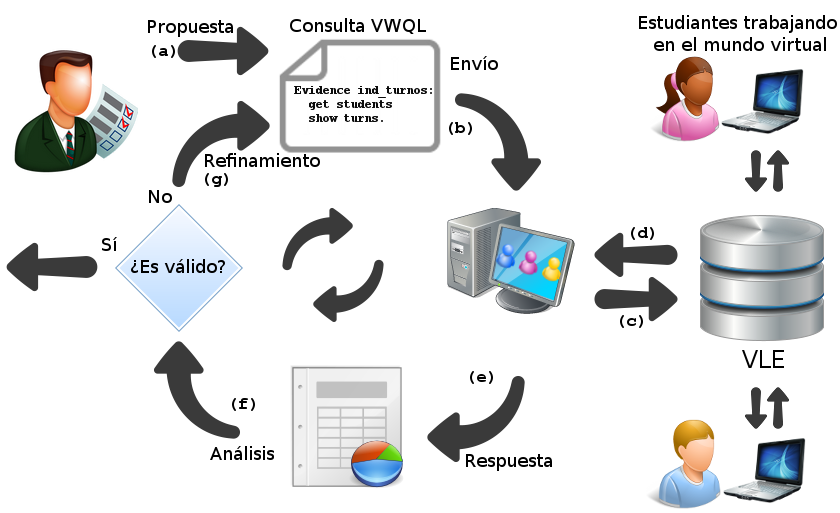
\includegraphics[scale=0.4]{EvsDiagram.png}
  \end{center}
  \caption{Ciclo de contraste de hipótesis con EvalSim}
  \label{fig:EvsDiagram}
\end{figure}

El profesor propone una evaluación (\emph{a}) que bajo su criterio le vaya a proporcionar indicadores válidos para evaluar alguna competencia genérica y la envía a EvalSim (\emph{b}). EvalSim procesa la petición y realiza la solicitud a la base de datos del mundo virtual (\emph{c}) . Una vez que recibe los datos (\emph{d}), los transforma y devuelve los resultados debidamente formateados al profesor (\emph{e}). El profesor los analiza, y si considera que son indicadores válidos para evaluar la competencia (\emph{f}) termina el ciclo. Sin embargo, si entiende que no les sirven o considera que debería refinarlo podría volver a diseñar una nueva evaluación (\emph{g}), reiniciándose de nuevo el ciclo.


\paragraph*{Ejemplo de uso}

En este ejemplo se parte de que el mundo virtual se está utilizando en una asignatura de idiomas. En un ejercicio práctico confeccionado por el profesor, los estudiantes han de participar en un juego de roles (\emph{role-play}) y son advertidos de que deben explayarse en sus respuestas a fin de utilizar los recursos lingüísticos aprendidos en clase.

Una vez que todos los estudiantes han participado el juego, el profesor decide utilizar como indicador el número de frases de una sola palabra utilizada por los estudiantes. De esta manera, todos aquellos estudiantes que hayan utilizado una sola palabra para responder a alguna pregunta tendrán una evaluación negativa en el desempeño de la competencia. Puede verse el código empleado en la consulta~\ref{code:vqwlej1}.

\begin{lstlisting}[caption=Respuestas de una sola palabra, label=code:vqwlej1,numbers=left, captionpos=b, morekeywords={Evidence,get, students, single, show, words, sentences, turns, time, points}]
Evidence respuestas_cortas:
    get students
    show single.
\end{lstlisting}

Como resultado a la consulta, el sistema devuelve el listado que puede verse en la tabla~\ref{tab:EvsListEj1}. A la vista de los mismos, el profesor considera que hay situaciones en las que una respuesta corta podría admitirse como válida, por lo que decide admitir como mucho dos respuestas cortas en la participación de cada estudiante. Ante este enfoque, el profesor considera que los estudiantes 3, 6 y 7 (\emph{studen3, student6 y student7}) tuvieron un desempeño bajo en la competencia al haber empleado cuatro, cuatro y tres respuestas cortas respectivamente.

\begin{table}
	\centering
	\caption{Información sobre las respuestas de una sola palabra dadas por los estudiantes en el role-play}
	\label{tab:EvsListEj1}
	\begin{tabular}{|l|l|c|}
		\hline
		id & username & singles \\
		\hline
		\hline
		1 & student1 & 0  \\
		\hline
		2 & student2 & 1  \\
		\hline
		3 & student3 & 4  \\
		\hline
		4 & student4 & 0  \\
		\hline
		5 & student5 & 2  \\
		\hline
		6 & student6 & 4  \\
		\hline
		7 & student7 & 3  \\
		\hline
		8 & student8 & 1  \\
		\hline
	\end{tabular}
\end{table}

Para enriquecer este indicador, el profesor decide diseñar un nuevo indicador. En este caso, calculando el número de palabras por turno que escriben los estudiantes. Para ello utiliza la consulta~\ref{code:vqwlej2}. Los resultados en este caso puede verse en la tabla~\ref{tab:EvsListEj2}.

\begin{lstlisting}[caption=Respuestas de una sola palabra, label=code:vqwlej2,numbers=left, captionpos=b, morekeywords={Evidence,get, students, single, show, words, sentences, turns, time, points}]
Evidence palabras_turno:
    get students
    show words, turns.
\end{lstlisting}

\begin{table}
	\centering
	\caption{Información sobre las palabras por turnos utilizadas por los estudiantes en el role-play}
	\label{tab:EvsListEj2}
	\begin{tabular}{|l|l|c|c|c|}
		\hline
		id & username & words & turns & words per turn \\
		\hline
		\hline
		1 & student1 & 117 & 9 & 13 \\
		\hline
		2 & student2 & 132 & 11 & 12  \\
		\hline
		3 & student3 & 63 & 9 & 7  \\
		\hline
		4 & student4 & 140 & 10 & 14  \\
		\hline
		5 & student5 & 99  & 11 & 9 \\
		\hline
		6 & student6 & 80 & 10 & 8  \\
		\hline
		7 & student7 & 72 & 9 & 8  \\
		\hline
		8 & student8 & 108 & 9 & 12   \\
		\hline
	\end{tabular}
\end{table}

A la vista de los resultados, el profesor confirma que los estudiantes 3, 6 y 7 (\emph{studen3, student6 y student7}) son los que utilizan menos palabras por turno. Son estos tres estudiantes, junto con el estudiante número 5 (\emph{student5}), los únicos que bajan de 10 palabras por turno. Lo que podría ser una justificación para el profesor a la hora de evaluar de manera negativa a este estudiante, ya que no sólo no llega a 10 mensajes sino que también es el único que en la consulta anterior está en el límite fijado de dos respuestas cortas.

Como en los casos anteriores, será decisión del profesor el uso que se dé a los indicadores.

\paragraph{Indicadores}

El mundo virtual se ha desarrollado para asignaturas de idiomas, por lo que la competencia genérica para la que más se han utilizado los indicadores obtenidos ha sido para la \emph{habilidad para comunicarse en un segundo idioma}. Aunque sólo es una propuesta y podrían utilizarse también para otras competencias.

% Hipótesis: un estudiante tiene dificultades para hacerse entender si necesita dos o más frases por turno para comunicarse con su compañero.

\paragraph*{Segundo idioma}
\begin{itemize}
\item \emph{Ritmo}: número de frases escritas por minuto. Según la experiencia desarrollada podría ser un indicador positivo o negativo del desempeño de la competencia. Si el estudiante tiene que contar una historia o expresarse sin restricción, el hecho de que escriba muchas frases por minuto es un indicador positivo de su dominio del idioma. Sin embargo, si el estudiante tiene que enviar a su compañero un mensaje concreto y tiene dificultades  para hacerse entender, puede necesitar más de una frase por minuto para hacerse entender, siendo entonces un indicador negativo.
\item \emph{Frases por turno}: número de frases escritas por turno. Igual que en el caso anterior, puede tomarse como un indicador positivo o negativo dependiendo del caso. Si el estudiante tiene un buen dominio del idioma y no hay restricción impuesta, puede ser un indicador positivo que escriba muchas frases por turno. Mientras que si necesita muchas frases para transmitir un mensaje concreto, que tenga que escribir muchas frases por turno puede ser un indicador negativo del desempeño de la competencia.
\item \emph{Palabras solas}: número de frases de una sola palabra escritas por el estudiante. Un abuso del uso de frases de una sola palabra puede ser utilizado como un indicador del bajo nivel de conocimiento del segundo idioma.
\end{itemize}

\paragraph*{Capacidad de aprender y mantenerse al día con el aprendizaje}
Si un estudiante tiene dificultades para desenvolverse en el idioma, el hecho de que dedicase muchos minutos a jugar en el mundo virtual podría ser un indicador de que dicho estudiante está comprometido con su aprendizaje, y quiere mejorar. Sin embargo, si un estudiante tiene malos resultados, y además pasa pocos minutos practicando, sería un indicador negativo de esta competencia.

% ---------------------------------------------------------------------
% ---------------------------------------------------------------------
% Fin entornos de aplicación
% ---------------------------------------------------------------------
% ---------------------------------------------------------------------

\subsection{Publicaciones}

Durante el desarrollo de este método se ha tratado de publicar en diferentes ámbitos a partir de cada una de sus implementaciones. La evaluación realizada en revistas de ímpacto y conferencias de relevancia son realizadas mediante procesos de \emph{revisión por par doble-ciego}, donde tanto los revisores como los autores son anónimos~\cite{ladron2008revision}. De esta forma se han recibido evaluaciones, opiniones y recomendaciones, que se han ido incorporando a las diferentes implementaciones y al método.

\subsection{Cuestionarios y entrevistas}

En el transcurso de esta tesis se ha presentado en varios foros el trabajo que se va desarrollando. Los profesionales de la educación que han asistido a las presentaciones han participado en cuestionarios de evaluación de la propuesta y han vertido sus opiniones y recomendaciones sobre el método en las entrevistas realizadas. Los profesionales que han participado son profesores universitarios, profesores de primaria y secundaria y personal de MediaWiki España.

% AMW ---------------------------------------------------------------------------------
\section{AMW aplicado a MediaWiki}

El estudio de caso donde se aplica por primera vez AMW se presentó en el \emph{SPEDECE 2012 (Ninth multidisciplinary symposium on the design and evaluation of digital content for education)}~\cite{Balderas:2012} y se amplió en la versión enviada a la revista Computers \& Education en 2015~\footnote{http://www.journals.elsevier.com/computers-and-education/}, pendiente aún de ser publicada.

\subsection{Evaluación}

El estudio de caso en el que se aplicó AMW tuvo lugar en la titulación de \emph{Ingenieria Técnica en Informática de Sistemas},  de la Universidad de Cádiz, en el curso 2011-12. La experiencia fue desarrollada en la asignatura de \emph{Administración de Sistemas Operativos} con 40 estudiantes matriculados. Dentro de las actividades de la asignatura se incluyó el desarrollo de un proyecto en el wiki, que fue evaluado mediante una aproximación mixta con SMW y AMW.

En una primera iteración del \emph{ciclo de contraste de hipótesis} se obtuvieron indicadores cuantitativos, mientras que en la segunda iteración los indicadores que se obtuvieron fueron cualitativos. 
Las dimensiones que se pretendían evaluar fueron las siguientes:

\begin{itemize}
	\item Trabajo en equipo ($M_1$)
	\item Comunicación y la aplicación del conocimiento ($M_2$)
	\item Habilidades individuales ($M_3$)
	\item Capacidad critica ($M_4$)
	\item Entregable final ($M_5$)
\end{itemize}

\subsubsection{Indicadores cuantitativos}

Para la evaluación de competencias en este primer ciclo se decidió partir de indicadores cuantitativos, midiendo en bytes la cantidad de trabajo realizada por cada estudiante en las contribuciones hechas al wiki. Para ela aplicación del método se usó SMW. Los indicadores que se utilizaron fueron los siguientes:

\begin{itemize}
	\item Trabajo en equipo ($M_1$): Ratio de miembros del equipo que contribuyeron en el proyecto wiki.
	\item Comunicación y la aplicación del conocimiento ($M_2$): Ratio de miembros del equipo que contribuyeron al menos a un 20\percentage del conteo final de bytes de la categoría.
	\item Habilidades individuales ($M_3$): contribución en bytes.
	\item Capacidad critica ($M_4$): No considerado
\end{itemize}

\subsubsection{Indicadores cualitativos}

En esta segunda iteración del \emph{ciclo de contraste de hipótesis} se utilizó AMW para obtener indicadores cualitativos. Había numerosos aspectos que se escapaban de la evaluación después de obtener los indicadores cuantitativos y que un análisis cualitativo complementaría. Los indicadores que se utilizaron en este caso para las competencias fueron los siguientes:

\begin{itemize}
	\item Trabajo en equipo ($M_1$): Ratio de miembros del equipo que trabajaron en el mismo criterio técnico.
	\item Comunicación y la aplicación del conocimiento ($M_2$): Media de las notas que los miembros del equipo recibieron.
	\item Habilidades individuales ($M_3$): Media de las notas que cada estudiante recibió.
	\item Capacidad critica ($M_4$): Número de evaluaciones que el estudiante realizó y que fueron posteriormente modificadas por el profesor.
\end{itemize}

\subsubsection{Resumen}

En la tabla~\ref{table:skill-assessed} puede verse una comparativa de los indicadores cuantitativos y cualitativos. Durante el análisis de los indicadores cuantitativos se detectaron pequeños defectos que tuvieron que ser completementados con indicadores cualitativos. 

\begin{table}[h]
\centering
\begin{tabular}{|m{3.1cm}|m{5cm}|m{5cm}|}
\hline
\textbf{Competencia} & \textbf{Indicadores cuantitativos} & \textbf{Indicadores cualitativos}   \\ \hline
\hline
Trabajo en equipo & Ratio de miembros del equipo que contribuyeron a la misma página wiki dentro del proyecto & Ratio de miembros del equipo que trabajaron en el mismo criterio técnico \\
\hline
Comunicación y aplicación del conocimiento & Ratio de miembros del equipo que contribuyeron al menos al 20\percentage del conteo final de bytes de la categoría  & Media de las notas que los miembros del equipo recibieron  \\
\hline
Habilidades individuales  & Contribución en bytes & Media de las notas que el estudiante recibió \\
\hline
Pensamiento  & & Número de evaluaciones que \\
crítico & \emph{No considerado} & el estudiante hizo y fueron \\
 & & modificadas por el profesor  \\
\hline
Entregable final & Manualmente & Manualmente \\
\hline
\end{tabular}
\caption{Resumen de indicadores para cada aproximación.}
\label{table:skill-assessed}
\end{table}

En la competencia de trabajo en equipo, con el enfoque cuantitativo, era muy sencillo para muchos estudiantes conseguir un indicador positivo, ya que por el simple hecho de haber escrito algo en la página era suficiente. Sin embargo, esto no justificaba en sí un trabajo en equipo, sino el haber trabajado algo, aunque fuese poco, en el mismo proyecto. Por ello se planteó el enfoque cualitativo. Al considerarse varios aspectos en un trabajo, y el estar estos aspectos representados en criterios de la rúbrica, el hecho de que dos o más estudiantes tuviesen alguna calificación en un mismo criterio podría considerarse como una evidencia de que esos estudiantes han trabajado en colaboración para alcanzar el objetivo representado en dicho criterio.

Para la competencia de la comunicación y la aplicación del conocimiento se consideró la cantidad de miembros del equipo que contribuyó al menos al 20\percentage de la versión final del wiki en términos de bytes. Este indicador evalúa el nivel de competencia de los equipos de trabajo que contribuyen al éxito del proyecto. Sin embargo, este indicador podía ser confuso. Si un estudiante mueve un trozo de texto considerable el sistema consideraría esta acción como una contribución importante cuando en realidad no lo merece. Incluso un estudiante podría engañar al sistema de pegando texto absurdo y borrándolo después, y así contribuir a unas cifras de trabajo que no serían reales pero que pasarían por alto en un análisis cuantitativo. Por eso, este indicador se complementó con un análisis cualitativo, en el que si un estudiante mueve un trozo de texto de un sitio a otro, quizás pueda obtener una beuan nota en el criterio de la coherencia del texto, pero desde luego no en un criterio específico. En este enfoque cualitativo, a partir de la media de todas las calificaciones de todas las contribuciones de los miembros del equipo se mide cómo han aplicado los estudiantes el conocimiento y cómo se han comunicado para este fin.

Para las competencias de las habilidades individuales nos encontramos ante la misma situación. Medir en bytes el trabajo de los profesores te aporta un dato cuantitativo válido, pero que necesita un análisis cualitativo que tenga en cuenta posibles situaciones que se tendrían en cuenta con el enfoque cuantitativo. Con la media de las calificaciones de las contribuciones realizadas individualmente por cada estudiante se complementa la evaluación de esta competencia.

Para el pensamiento crítico se tiene en cuenta sólo el aspecto cualitativo. Los estudiantes disponen del conocimiento para realizar la evaluación del trabajo de sus compañeros. Los estudiantes evaluados pueden reclamar una evaluación recibida si no están de acuerdo con la misma. En ese caso es el profesor el que se encarga de la revisión, y si modifica la nota, el alumno evaluador será penalizado en esta competencia.

\subsection{Resultados}
La experiencia constaba de las tres fases que fueron introducidas en el capítulo anterior:

\begin{description}
\item[1. Desarrollo del trabajo en el wiki]

Esta etapa se inició con un seminario donde los estudiantes aprendieron cómo debían trabajar colaborativamente en un wiki basado en MediaWiki. Después, los estudiantes se dividieron en doce grupos de tres miembros y dos grupos de dos miembros. Cada grupo tuvo que escribir la documentación de su proyecto en una sola página wiki. Dado que uno de los objetivos de la asignatura era desarrollar una experiencia de \emph{evaluación auténtica}, el cometido del proyecto era la planificación y gestión del proceso de migración real de un sistema de información de la empresa. Los estudiantes fueron los responsables de la planificación y la gestión de su asignación, la coordinación de sus tareas y del trabajo en colaboración. El wiki está disponible públicamente~\footnote{http://wikis.uca.es/wikiASO/}, y en seis semanas de los estudiantes crearon más de 1.400 ediciones en los 14 proyectos que participaron en la asignatura. Como guía de esta experiencia, mostraremos los resultados obtenidos por los cuatro grupos de tres miembros de la tabla~\ref {tab:AmwGroupsMembers}.

\begin{table}[h]
\centering
\begin{tabular}{|c|c|}
\hline
\textbf{Project ($P_i$)} & \textbf{Members ($U_i$)}   \\ \hline
\hline
 $P_1$ & $U_7$, $U_8$, $U_9$  \\ \hline
 $P_4$ & $U_{13}$, $U_{14}$, $U_{15}$  \\ \hline
 $P_7$ & $U_4$, $U_5$, $U_6$  \\ \hline
 $P_{13}$ & $U_1$, $U_2$, $U_3$  \\ \hline
\end{tabular}
\caption{Grupos de ejemplo y sus miembros.}
\label{tab:AmwGroupsMembers}
\end{table}

\item[2. Evaluación de los estudiantes]

Esta fase comenzó con un seminario. Los estudiantes aprendieron cómo evaluar contribuciones al wiki mediante el uso de AMW. Tras ello, los estudiantes realizaron 412 evaluaciones cualitativas de contribuciones al wiki. Este proceso proporcionó a los estudiantes información crítica sobre su trabajo. Los estudiantes también pudieron replicar una evaluación si no estaban de acuerdo con la misma.

\item[3. Revisión del profesor]

El profesor tuvo que resolver las réplicas. Esta información se utilizó más tarde para evaluar el pensamiento crítico.

\end{description}

AMW se utilizó para evaluar el desempeño de los estudiantes en varios indicadores relacionados con el trabajo en equipo. Indicadores como la coordinación para desempeñar tareas y su desempeño de manera colaborativa. Además, se fomento el pensamiento crítico de los estudiantes motivándoles a revisar formalmente el trabajo de sus compañeros para que su nota no se bajase.

A continuación en cada subsección se explica cómo se evaluaron las competencias para cada subdimensión. Esta propuesta se basa en el programa de la asignatura. Dependiendo de la configuración de las tareas específicas del wiki y de la actividad a desarrollar, el profesor podría utilizar estos indicadores como proponemos, adaptarlos a la evaluación de otras habilidades, o incluso definir sus indicadores.

\subsubsection{Indicador del trabajo en equipo ($M_1$)}

\paragraph*{Aproximación cuantitativa}

Mediante el uso de SMW se pudo comprobar como todos los miembros de cada equipo, en menor o mayor medida habían participado en la páginas wikis de sus proyectos. Este indicador se descartó, ya que una vez analizado lo único que podíamos saber era si los estudiantes habían contribuido al proyecto, pero el hecho de haber contribuido al mismo proyecto no es necesariamente una evidencia de haber trabajado en equipo. Por tanto, este indicador se redifinió mediante la aproximación cualitativa.

\paragraph*{Aproximación cualitativa}

Esta calificación mide la habilidad de un equipo para trabajar colaborativamente y era compartida por todos los miembros del equipo ($U_i$) de cada proyecto ($P_i$). Esta dimensión recogía los criterios en los que fue evaluado cada $U_i$ en la página de su proyecto. Consideramos que un $U_i$ ha contribuido en un criterio de un proyecto si ha sido evaluado en ese criterio en alguna de sus contribuciones.

De esta forma, dos o más estudiantes colaboraron si fueron evaluados en el mismo criterio. Si dos miembros del equipo fueron evaluados en criterios complementarios, ello no implicaba colaboración. Bajo esta premisa sólo se consideraron los criterios técnicos, que están relacionados con las partes de la tarea en la que los estudiantes en realidad colaboraron. La colaboración en criterios transversales como la escritura o la coherencia no se consideraron ($D_{11}$-$D_{17}$).

En la tabla~\ref{table:13-project-grades} se muestran los criterios evaluados para cada miembro del proyecto $P_{13}$. Mientras que $U_1$ fue evaluado en cinco criterios, $U_2$ y $U_3$ sólo fueron evaluados de uno. Los criterios \emph{servidor físico} ($D_4$) , \emph{red} ($D_6$) , \emph{PCs} ($D_7$) , \emph{Gantt} ($D_9$) y \emph{presupuesto} ($D_10$) sólo fueron trabajados por un miembro del equipo ($U_1$). El único criterio trabajado por más de un miembro del equipo fue $D_8$, que fue trabajado por $U_1$ y $U_2$. Así que, bajo nuestra propuesta, $U_1$ y $U_2$ trabajaron colaborativamente, pero $U_3$ no.

\begin{table}[h]
\centering
\begin{tabular}{|c|c|c|c|c|c|c|c|c|c|c|l|}
\hline
\textbf{Estudiante} & \textbf{$D_1$} & \textbf{$D_2$} & \textbf{$D_3$} & \textbf{$D_4$} & \textbf{$D_5$} & \textbf{$D_6$} & \textbf{$D_7$} & \textbf{$D_8$} & \textbf{$D_9$} & \textbf{$D_{10}$} & \textbf{Collaboración} \\ \hline
\hline
$U_1$ &   &   &   & 1 &   &     & 1   & \textbf{1}  & 1  & 1  & \textbf{sí (en $D_8$ con $U_2$)} \\ \hline
$U_2$ &   &   &   &    &   &     &      & \textbf{1}    &      &       & \textbf{sí (en $D_8$ con $U_1$)} \\ \hline
$U_3$ &   &   &   &    &   & 1  &     &      &      &       & \textbf{no} \\ \hline
% \hline
% \hline
% Sum &   &   &   & 1 &   & 1  & 1   & \textbf{2}  & 1  & 1  & \textbf{2 out of 3} \\ \hline
% \hline\multicolumn{13}{|c|}{\textbf{1 out of 3 $\rightarrow$ 33.3\% $\rightarrow$ \underline{3.33 out of 10}}} \\ \hline
\end{tabular}
\caption{Grading of collaborative work ($M_1$) in the $P_{13}$ project.}
\label{table:13-project-grades}
\end{table}

Finalmente, la calificación del grupo en esta dimensión se calculaba con la fórmula~\ref{math:m1}. 

\begin{equation}
    \textbf{$M_1 = CTM/TM$}
    \label{math:m1}
\end{equation}

En dicha fórmula participan las siguientes variables:

\begin{itemize}	
	\item \emph{CTM (collaborative team members}: número de miembros del equipo que trabajaron colaborativamente.
	\item \emph{TM (team members)}: número de miembros que componen el equipo.
\end{itemize} 

La calificación $M_1$ para el proyecto $P_{13}$ fue de 6,66 sobre 10, ya que dos de los tres miembros trabajaron colaborativamente.

\subsubsection{Indicador de las habilidades de comunicación y la aplicación del conocimiento ($M_2$)}

\paragraph*{Aproximación cuantitativa}

En este enfoque se considera la cantidad de miembros de cada equipo que habían contribuido al menos a un 20\percentage del trabajo realizado en la página del wiki medido en bytes (para equipos de tres estudiantes). En la figura~\ref{fig:smw-p13} puede verse una gráfica de la distribución del trabajo, mostrándose el ratio total de bytes contribuidos por cada estudiante del proyecto $P_{13}$. $U_1$ (verde) contribuyó con un 38,2\percentage, $U_2$ (rojo) con un 27,2\percentage y $U_3$ (azul) con un 34,7\percentage. Al estar más o menos balanceada consideramos que ellos trabajaron colaborativamente.

\begin{figure}
	\centering
	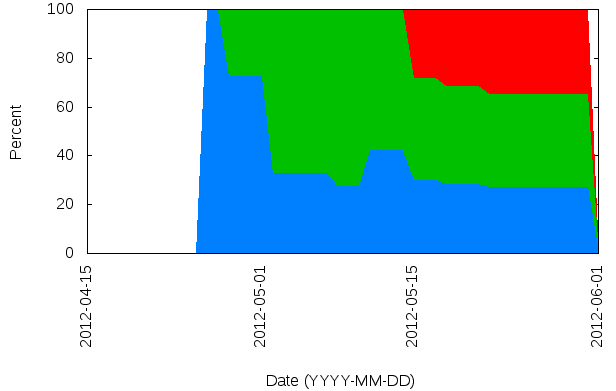
\includegraphics[width=8cm]{smw-work-distribution-p13.png}
	\caption{Distribución del trabajo de los miembros del proyecto $P_{13}$.}
	\label{fig:smw-p13}
\end{figure}

\paragraph*{Aproximación cualitativa}

Esta calificación medía la habilidad para aplicar el conocimiento en situaciónes prácticas y la habilidad para comunicarse con otros miembros del equipo. La calificación de este indicador también era compartida por todos los miembros del equipo ($U_i$). Se calcula como la media de las notas que cada miembro del equipo recibió. Este indicador evaluaba la eficacia de los equipo de trabajo que contribuyen al éxito del proyecto. Notas medias en las contribuciones pueden significar pobres contribuciones al wiki o que algunas contribuciones obtuvieron buenas calificaciones y otras malas, evidenciando una comunicación deficiente entre los miembros del equipo o un escaso grado de compromiso con el equipo.

La media de todas las calificaciones dadas a los criterios de cada contribución a los miembros de cada equipo en el proyecto se calcula mediante la fórmula~\ref{math:m2}.

\begin{equation}
    \textbf{$M_2 = SRA_G/NRA_G$}
    \label{math:m2}
\end{equation}

En dicha fórmula participan las siguientes variables:
\begin{itemize}	
	\item \emph{$SRA_G$ (sum of received assessments)}: suma de las calificaciones recibidas para todas las contribuciones del proyecto.
	\item \emph{$NRA_G$ (number of received assessments)}: número de evaluaciones recibidas.
\end{itemize} 

\begin{table}[h]
\centering
\begin{tabular}{|c|r|r|r|r|r|r|r|r|r|r|r|r|r|}
\hline
\textbf{Estudiante} & \textbf{$D_1$} & \textbf{$D_2$} & \textbf{$D_3$} & \textbf{$D_4$} & \textbf{$D_5$} & \textbf{$D_6$} & \textbf{$D_7$} & \textbf{$D_8$} & \textbf{$D_9$} & \textbf{$D_{10}$} & \textbf{$D_{11}$} &  \textbf{$SRA_G$ } & \textbf{$NRA_G$ } \\ \hline
\hline
$U_4$ & 15  & 13  & 7  & 26 & 22 & 34  & 30 & 6   & 25  & 37 & 89  & \textbf{304} & \textbf{40} \\ \hline
$U_5$ &      &      &     & 26 & 8   &      &      &      &  18 &      & 17 &  \textbf{69}  & \textbf{8} \\ \hline
$U_6$ &     &  8    &    &  25 & 9  &     &   7   &  8   &      &  8  &  133 & \textbf{198} & \textbf{26} \\ \hline
\hline
\hline
\multicolumn{12}{|r|}{\textbf{Suma}} & 571 &  74 \\ \hline
\multicolumn{12}{|r|}{\textbf{Media}} & \multicolumn{2}{|c|}{\textbf{7.71}} \\ \hline
\end{tabular}
\caption{($M_2$) para el proyecto $P_{7}$.}
\label{table:7-project-peers-grades}
\end{table}

\begin{table}[h]
\centering
\begin{tabular}{|c|r|r|r|r|r|r|r|r|r|r|r|r|r|}
\hline
\textbf{Estudiante} & \textbf{$D_1$} & \textbf{$D_2$} & \textbf{$D_3$} & \textbf{$D_4$} & \textbf{$D_5$} & \textbf{$D_6$} & \textbf{$D_7$} & \textbf{$D_8$} & \textbf{$D_9$} & \textbf{$D_{10}$} & \textbf{$D_{11}$} &  \textbf{$SRA_G$ } & \textbf{$NRA_G$ } \\ \hline
\hline
$U_{13}$ &   &   &   & 24 &      & 15  & 7   & 7   & 8   & 47  & 98  & \textbf{206} & \textbf{27} \\ \hline
$U_{14}$ &   &   &   & 26 & 8   &      &      &      &  27 &      & 10 &  \textbf{37}  & \textbf{4} \\ \hline
$U_{15}$ & 22 &  46 & 21   &  40 & 17  & 5 & 94 &  5   & 6  &  20  &  123 & \textbf{399} & \textbf{64} \\ \hline
\hline
\hline
\multicolumn{12}{|r|}{\textbf{Suma}} & 642 &  95 \\ \hline
\multicolumn{12}{|r|}{\textbf{Media}} & \multicolumn{2}{|c|}{\textbf{6.75}} \\ \hline
\end{tabular}
\caption{$M_2$  para el proyecto $P_{4}$.}
\label{table:4-project-peers-grades}
\end{table}

% Dejo la parte cuantitativa??
%Para la evaluación cuantitativa se consideró la cantidad de miembros del equipo que contribuyeron al menos a un 20\percentage de los bytes de la versión final del wiki (para equipos de tres estudiantes). En la figura~\ref{} puede verse una gráfica de la distribución del trabajo, mostrándose el ratio total de bytes contribuidos por cada estudiante del proyecto $P_{13}$. $U_1$ (verde) contribuyó con un 38,2\percentage, $U_2$ (rojo) con un 27,2\percentage y $U_3$ (azul) con un 34,7\percentage. Al estar más o menos balanceada consideramos que ellos trabajaron colaborativamente.

\subsubsection{Indicador de habilidades individuales ($M_3$)}

\paragraph*{Aproximación cuantitativa}

bla bla bla

\paragraph*{Aproximación cualitativa}

Esta dimensión evalúa la capacidad para producir y mantener la calidad del proyecto. Es una habilidad individual, y se calcula por separado para cada miembro del equipo ($U_i$). El grado en esta dimensión es el promedio de las calificaciones recibidas para cada alumno, expresado en la fórmula~\ref{math:m3}.

\begin{equation}
    \textbf{$M_3 = SRA_S/NRA_S$}
    \label{math:m3}
\end{equation}

En dicha fórmula participan las siguientes variables:
\begin{itemize}	
	\item \emph{$SRA_S$ (sum of received assessments by the student)}: suma de las calificaciones recibidas para las contribuciones del estudiante.
	\item \emph{$NRA_S$ (number of received assessments by the student)}: número de evaluaciones recibidas por el estudiante.
\end{itemize} 

El promedio de las calificaciones asignadas a las contribuciones de cada estudiante del proyecto $P_4$ ($U_{13}$, $U_{14}$, $U_{15}$) y del proyecto $P_{13}$ ($U_1$, $U_2$, $U_3$) puede verse en la tabla~\ref{table:project-individual-grades}. Bajo nuestro enfoque, los miembros de $P_{13}$ tuvieron calificaciones similares. Pero en $P_4$ puede verse un constraste, ya que $U_{14}$ hizo buenas aportaciones, mientras que $U_{15}$ no contribuyó a la calidad del proyecto.

\begin{table}[h]
\centering
\begin{tabular}{|c|c|r|r|r|r|r|r|r|r|r|r|r|r|r|r|}
\hline
\textbf{$P_i$} & \textbf{$U_i$} & \textbf{$D_1$} & \textbf{$D_2$} & \textbf{$D_3$} & \textbf{$D_4$} & \textbf{$D_5$} & \textbf{$D_6$} & \textbf{$D_7$} & \textbf{$D_8$} & \textbf{$D_9$} & \textbf{$D_{10}$} & \textbf{$D_{11}$} &  \textbf{$SRA_G$ } & \textbf{$NRA_G$ } & \textbf{$M_3$} \\ \hline
\hline
\multirow{3}{*}{$P_{13}$} & $U_1$ &   &   &   & 7 &   &     & 15   & 13  & 16  & 40  & 24 & 115 & 15 & 7.67 \\
 & $U_2$ &   &   &   &    &   &     &      & 8    &      &       &     & 8    & 1   & 8.00 \\
 & $U_3$ &   &   &   &    &   & 14  &     &      &      &       & 15 &  29 & 4   & 7.25  \\ \hline
 & $U_{13}$ &   &   &   & 24 &      & 15  & 7   & 7   & 8   & 47  & 98  & \textbf{206} & \textbf{27} & 7.62 \\ 
 & $U_{14}$ &   &   &   & 26 & 8   &      &      &      &  27 &      & 10 &  \textbf{37}  & \textbf{4} & 9.25 \\ 
\multirow{-3}{*}{$P_{4}$} & $U_{15}$ & 22 &  46 & 21   &  40 & 17  & 5 & 94 &  5   & 6  &  20  &  123 & \textbf{399} & \textbf{64} & 6.23 \\ \hline
\end{tabular}
\caption{($M_3$) para los miembros de $P_{4}$ y $P_{13}$.}
\label{table:project-individual-grades}
\end{table}

% Cuantitativo?

\subsubsection{Indicador del pensamiento crítico ($M_4$)}

\paragraph*{Aproximación cuantitativa}

bla bla bla

\paragraph*{Aproximación cualitativa}

Como se ha comentado anteriormente, AMW permitió a los estudiantes replicar si estabán en desacuerdo con una evaluación recibida. Esas réplicas se reportaron al supervisor para resolverlos. En caso de que el profesor aceptase una réplica, la calificación se modificaba. Pero este proceso tiene otra parte: los estudiantes recibieron instrucciones claras sobre la tarea de evaluación, siendo un proceso formativo que tenía reflejo en su calificación. Entonces, podíamos utilizar esta información como un indicador de la habilidad para \emph{interpretar, analizar y evaluar el trabajo de sus compañeros}. En particular, hemos utilizado dos indicadores: el número de evaluaciones realizadas por cada estudiante y la cantidad de ellos que el profesor modificó (podían tener su origen en réplicas del estudiante evaluado o en revisiones al azar realizadas por el profesor). No fue nuestro caso, pero si había diferentes evaluaciones en una misma contribución, la diferencia entre ellos podría ser también un indicador de competencia.

La fórmula que se utilizó fue~\ref{math:m4}. Se considera que todos los estudiantes comenzaron con 10 puntos en esta dimensión, y perdieron 2,5 de ellos por cada evaluación que hicieron  y que fue modificado por el profesor, hasta un mínimo de 0 puntos. De hecho, cada estudiante hizo 10 evaluaciones, por lo que consideramos que deberían haber hecho no más del 20\percentage de las evaluaciones erróneas para aprobar esta parte de la nota. En nuestro caso de estudio, tuvimos 412 evaluación, y 27 de ellas (6\percentage) se replicaron (el profesor sólo revisó las evaluaciones replicadas). Sólo 10 de ellas (37\percentage) fueron aceptadas. En cuanto a los estudiantes, sólo uno tuvo 3 réplicas a sus evaluacones aceptadas. El resto de ellos tenía 2, 1 o ninguno. En la tabla~\ref{table:students-grade-replies} pueden verse las evaluaciones realizadas por los miembros de $P_{13}$ que fueron respondidas. $U_1$ y $U_2$ recibieron una réplica que fue aceptada ($AR$) cada uno, mientras que $U_3 $ no tuvo ninguna.

\begin{equation}
    \textbf{$M_4 = 10 - 2.5 * AR$}
    \label{math:m4}
\end{equation}

\begin{table}[h]
\centering
\begin{tabular}{|c|c|c|c|}
\hline
\textbf{Students} & \textbf{Received replies} & \textbf{Accepted replies} & \textbf{$M_4$}  \\ \hline
\hline
 $U_1$ & 2 & 1 & 7.50  \\ \hline
 $U_2$ & 1 & 1 & 7.50 \\ \hline
 $U_3$ & 0 & 0 & 10.00  \\ \hline
\end{tabular}
\caption{($M_4$) para los miembros del proyecto $P_{13}$.}
\label{table:students-grade-replies}
\end{table}

\subsubsection{Entregable final ($M_5$)}

Para la calificación fina se tomó el trabajo final del wiki, donde se valoraron todos los requisitos que se esperaban del trabajo. En nuestro enfoque, cada $P_i$ tuvo una calificación entre 0-10. Esta fue la calificación dada por el profesor una vez se ha llegado a la fecha límite. La calificación fue la misma para todos los miembros del equipo ($U_i$), ya que todos ellos (como equipo) son responsables del resultado final del proyecto. Los proyectos fueron evaluados usando la rúbrica indica en el cuadro~\ref{table:project-rubric-supervisor}. Hay dos categorías de criterios en las rúbricas:

\begin{itemize}
\item Criterios específicos: atributos desde $D_1$ a  $D_{10}$, que se refieren a aspectos específicos del trabajo. 
\item Criterios transversales: atributos desde $D_{11}$ a  $D_{17}$, que se refieren a aspectos transversales del trabajo: coherencia, correcto uso del formato wiki, ... etc.
\end{itemize}

\begin{table}[h]
\centering
\begin{tabular}{|c|l|r|r|}
\hline
\textbf{Item} & \textbf{Criterios}  & \textbf{Peso}  & \textbf{Nota ($P_{13}$) }   \\ \hline
\hline
 $D_1$ & Justificación &  2.00 & 2.00 \\ \hline
 $D_2$ & Centro de datos anterior &   0.25 & 0.25 \\ \hline 
 $D_3$ & Centro de datos nuevo &    0.25 & 0.25 \\ \hline 
 $D_4$ & Servidor físico &    0.25 & 0.25  \\ \hline
 $D_5$ & Servidor virtual &    0.25 & 0.25  \\ \hline 
 $D_6$ & Red &    0.50 & 0.50  \\ \hline 
 $D_7$ & PCs &  0.40 & 0.40  \\ \hline 
 $D_8$ & Formación &    0.25 & 0.25  \\ \hline 
 $D_9$ & Diagrama de Gantt &    0.40  & 0.20  \\ \hline
 $D_{10}$ & Presupuesto &   0.40  & 0.40 \\ \hline
 $D_{11}$ & Escritura &   0.30  & 0.30 \\ \hline
 $D_{12}$ & Coherencia &   3.00  & 2.40 \\ \hline
 $D_{13}$ & Referencias &    0.25  & 0.00 \\ \hline
 $D_{14}$ & Formato wiki &    0.50  & 0.50 \\ \hline
 $D_{15}$ & Aplicación de conceptos teóricos &    1.00  & 0.50 \\ \hline
 $D_{16}$ & Información extra &    1.00  & 0.00 \\ \hline
 $D_{17}$ & Plagio &    -10.00  & -0.00 \\ \hline
 \hline
 \multicolumn{2}{|c|}{\textbf{Suma}} & \textbf{(Máx.) 10.00} & \textbf{8.45} \\ \hline
\end{tabular}
\caption{Calificaciones dadas por el profesor al proyecto $P_{13}$.}
% \caption{Grades the supervisor gave to the $P_{13}$ project using the rubric for the final version of the wiki pages.}
\label{table:project-rubric-supervisor}
\end{table}

A modo de ejemplo, la cuarta columna de la tabla muestra las calificaciones que el supervisor le dio a los criterios del proyecto $P_{13}$. Este proyecto fue calificado con un 8,45 puntos sobre 10. Esta evaluación cualitativa manual realizada por el supervisor es escalable, ya que cada grupo solo tiene una versión definitiva de su página wiki.

\subsection{Discusión} % Dejar? Eran resultados ...

Junto con el estudio de caso, varias comparaciones entre el enfoque cuantitativo previo y la cualitativa implementada en esta experiencia han sido desplegados. Un resumen sobre las ventajas del enfoque cualitativo se muestra a continuación:

\begin{itemize}
\item El enfoque cualitativo permite un análisis más fino de grano de trabajo colaborativo en comparación con los que en el experimento cuantitativo anterior.
\item Además, este análisis también puede detectar a los estudiantes que colaboran con un objetivo común en las diferentes páginas del wiki de un mismo proyecto.
\item Este enfoque permite la detección de las contribuciones que copiar, borrar y pegar de grandes fragmentos de texto sin tener que mejorar la página wiki, lo que podría tener una buena medición cuantitativa inmerecida.
\item Las contribuciones a otros proyectos se incluyen en la calificación individual de los estudiantes, mientras que estas contribuciones fueron de grano grueso en cuenta en el enfoque cuantitativo anterior.
\item La capacidad de los estudiantes para ser crítico es entrenado y evaluado por el proceso de respuesta.
\end{itemize}

Mientras que las principales desventajas son las siguientes:

\begin {itemize}
\item La función de selección debe ser cuidadosamente elegido, por lo que las evaluaciones se llevan a cabo en las contribuciones significativas.
\item Revisión de todas las evaluaciones de los compañeros y auto realizados por los estudiantes sigue siendo una tarea difícilmente escalable para el supervisor. Por lo tanto, algunas evaluaciones pobres pueden no detectados por el supervisor si no se informan, ni eligieron al azar para ser revisado.
\end {itemize}

En líneas generales, los estudiantes tuvieron un buen desempeño en la tarea. En la tabla~\ref{table:summary-theory} puede verse como solo 3 estudiantes no aprobaron el proyecto ($6.98\%$). Sin embargo, 37 estudiantes ($86.04\%$) tuvieron una buena calificación, más de 7 sobre 10. Los estudiantes llevaron a cabo tareasde análisis crítico mediante la evaluación del trabajo de sus compañeros. Así, obtuvieron retroalimentación y evidencias para cada evaluación recibida.

\begin{table}[h]
\centering
\begin{tabular}{|c|c|r|}
\hline
\textbf{Notas} & \textbf{Estudiantes} & \textbf{Ratio}   \\ \hline
\hline
 [9-10] & 16 & 37.21\% ~ \\ \hline
 [8-9) & 10 & 23.25\% ~ \\ \hline
 [7-8) & 11 & 25.58\% ~ \\ \hline
 [6-7) & 3 & 6.98\% ~ \\ \hline
 [5-6) & 0 & 0\% ~ \\ \hline
 [0-5) & 3 & 6.98\% ~ \\ \hline
\end{tabular}
\caption{Resumen de calificaciónes finales de los estudiantes}
\label{table:summary-theory}
\end{table}

%It is interesting to underline that the best peer-assessed grades were received by those students who were assessed fewest times. In particular there are only two students that had a grade average of 10, and they only had 1 and 3 assessments respectively. In fact, the following maximum one was 9.25, an average obtained by two students, both with 4 assessments. This was probably because they wrote large and very polished contributions. When their peers assessed them, they gave a very good grade because of the amount and quality of the information added. The only issue with these students is that they did not probably work collaboratively, and as a consequence had a lower grade in this dimension. This makes sense: if a student focuses on doing very few and large editions their mates can have problems to collaborate with them: they log in the wiki, contributes (a nice piece of text) and leave. So any issue of coherence with the rest of the project, or rewriting to adapt to change must be done by other team members (or it could even remain undone in the final version of the wiki page).


%Finally, 21 out of the 412 assessments (5\%) were self-assessment. The 85.71\% of these grades were between 8 and 9, and only one was below 5. After manually checking some of them, we have to acknowledge that were well assessed, although they weren't as severe with themselves as with their peers. Perhaps in a future case study every self-assessment should be automatically noticed to the supervisor to be checked and, eventually, could be considered an evidence of self-critical skill.

%Additionally, we could also detect the group organization, i.e. the roles adopted by each member. This was done by aggregating the criteria that each group member worked. This way we can identify groups where each member focused on different criteria. This is not necessarily bad if the final version of the wiki page is good. But in case it was not, it would be an evidence of a problem in group internal dynamics: probably each member did their work and nobody cared of relating individual parts to produce a coherent deliverable in the wiki. We could check the talk pages (both of the project pages and users ones) to see if they communicated and, in that case, the role that each member played.


% EVALCOURSE ---------------------------------------------------------------------------------
\section{EvalCourse aplicado a entornos de apredizaje virtual}

Los estudios de caso que se presentan en este capítulo fueron publicados en la revista~\emph{International Journal of Engineering Education, Special issue on Innovative Methods of Teaching Engineering}~\cite{Balderas:2015}, después de haber sido invitados a extender un primer trabajo presentado en el~\emph{4th International Workshop on Software Engineering for E-learning (ISELEAR’13)}~\cite{balderas2013generative}.

\subsection{Evaluación}

Los estudios de caso en los que se aplicó EvalCourse tuvieron lugar en dos asignaturas de la titulación de \emph{Ingenieria Informática}, de la Universidad de Cádiz, en el curso 2012/13. La evaluación del curso se realizó de forma manual, y después se aplicó EvalCourse para evaluar a los estudiantes en las competencias de liderazgo, habilidades interpersonales y el pensamiento crítico.

\subsubsection{Extracción de indicadores del foro}

El primero de los casos de estudio tuvo lugar en la asignatura de \emph{Procesadores de Lenguajes II} y que tenía 36 estudiantes matriculados. Era una asignatura obligatoria, que tenía lugar en el primer semestre del quinto (y último) curso. Durante el semestre, los estudiantes tuvieron que trabajar en pequeños equipos de dos o tres miembros. Cada equipo del curso tenía un foro para la comunicación interna. Este foro se utilizó para evaluar dos competencias: habilidades interpersonales y liderazgo.

En primer lugar, como indicador de las habilidades interpersonales de cada estudiante se calculó el total de intervenciones en el foro. El coordinador del curso animó a sus estudiantes a participar en el foro del equipo, ya que debía ser su herramienta de comunicación interna. Un estudiante que tenía tres o más intervenciones en el foro tendría una buena calificación. En segundo lugar, como indicador de liderazgo se consideró los debates que los estudiantes iniciaron en el foro. Un estudiante que inició dos o más debates tuvo una calificación positiva en la competencia de liderazgo.

\paragraph*{Análisis}

Sólo 18 de los 36 estudiantes del curso participaron en los foros. No se puede determinar que los estudiantes que no participaron en el foro no posean las competencias, lo único que podemos afirmar es que no demostraron su desempeño en estas competencias a través de esta actividad. Los resultados de haber aplicado EvalCourse pueden verse en el listado de la tabla~\ref{tab:EvcEvaluacionListadoForo1}. Pocos estudiantes obtuvieron una calificación positiva en estas competencias, habiendo varios estudiantes que destacan sobre el resto. Estos datos se exportaron a una hoja de cálculo y se genero la figura~\ref{fig:EvcEvaluacionTartaForo1}. En resumen, consideramos que los estudiantes, a pesar de que sabían que debían utilizar el foro para la comunicación entre los miembros del equipo, no lo hicieron en su mayoría.

\begin{table}
	\centering
	\caption{Listado de intervenciones de los estudiante en el foro.}
	\label{tab:EvcEvaluacionListadoForo1}
	\begin{tabular}{|c|l|c|c|c|}
		\hline
		id & username & Debate- & Debate- & Total  \\
			&		&	starter	& participation		&		\\
		\hline
		\hline
		43 &	S2 &	0 &	1 &	 1 \\
		44 &	S3 &	3 &	4 &	 7 \\
		45 &	S4 &	2 &	2 &	 4 \\
		46 &	S5 &	0 &	1 &	 1 \\
		48 &	S7 &	4 &	3 &	 7 \\
		50 &	S9 &	6 &	8 &	 14 \\
		51 &	S10 &	1 &	1 &	 2 \\
		53 &	S12 &	0 &	1 &	 1 \\
		55 &	S14 &	1 &	1 &	 2 \\
		59 &	S18 &	1 &	2 &	 3 \\
		60 &	S19 &	2 &	0 &	 2 \\
		61 &	S20 &	0 &	2 &	 2 \\
		62 &	S21 &	0 &	1 &	 1 \\
		67 &	S26 &	0 &	1 &	 1 \\
		70 &	S29 &	0 &	1 &	 1 \\
		71 &	S30 &	2 &	1 &	 3 \\
		75 &	S34 &	1 &	5 &	 6 \\
		78 &	S37 &	2 &	4 &	 6 \\
		\hline
	\end{tabular}
\end{table}

\begin{figure}
	\centering
	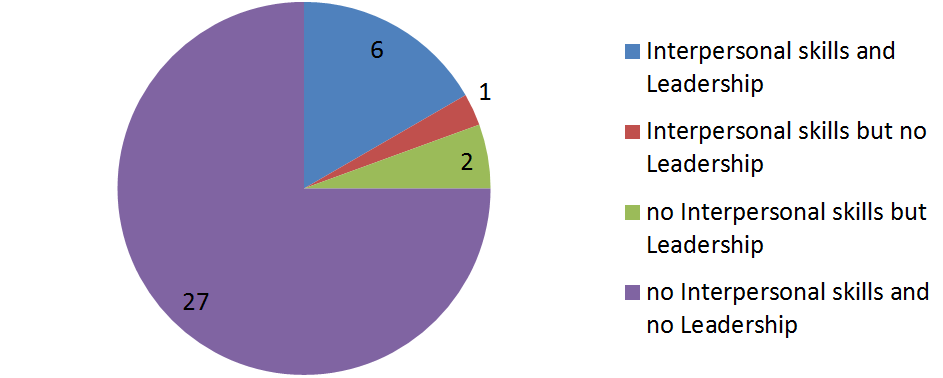
\includegraphics[width=12cm]{EvcForo1.png}
	\caption{Resumen del desempeño de los estudiantes en el foro en las dos competencias.}
	\label{fig:EvcEvaluacionTartaForo1}
\end{figure}

A pesar de esto, de manera informal sí se observó que los estudiantes con calificaciones positivas en ambas competencias realmente tuvieron un buen desempeño de dichas competencias en la asignatura. Por tanto, pudimos decir que los indicadores elegidos parecían ser verdaderas evidencias del nivel de competencia de los estudiantes. Probablemente el hecho de que el varlos dado a la participación en el foro en la calificación global de la asignatura fuera sólo de un 2,5\percentage no animó a los estudiantes a no utilizar en exclusiva sus habituales métodos de comunicación (Whatsapp, correo electronico, reuniones en el pasillo, etc.).

También se utilizó EvalCourse para analizar la interacción entre los estudiantes. La idea era localizar interacciones que quizás estuviese más interesadas en mejorar sus resultados que en la mera comunicación. Se detectaron evidencias de interacciones fraudulentas entre dos estudiantes cuando se podía ver que ellos sólo estaban interesados en hablar entre ellos dos y no habían interactuado con ningún otro compañero. Con el código SASQL mostrado en la consulta~\ref{code:interaction1} se obtuvo la interacción que hubo en el foro. Los resultados se pueden ver en la figura~\ref{fig:EvcEvaluacionInteraccionForo2}.


\begin{lstlisting}[caption=Código SASQL para extraer datos sobre la interacción en el foro ,label=code:interaction1,numbers=left, captionpos=b, morekeywords={Evidence,get, students, show, milestones, participation, access, in, assignment, forum, campus, workshop, interaction}]
Evidence forum_interaction: 
	get students
	show interaction
	in forum.
\end{lstlisting}

\begin{figure}
	\centering
	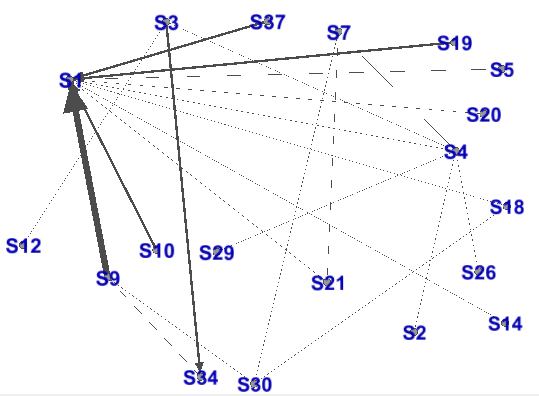
\includegraphics[width=12cm]{EvcForo2.png}
	\caption{Graph of students' interaction in forum case study.}
	\label{fig:EvcEvaluacionInteraccionForo2}
\end{figure}

Concluímos que gran parte de la interacción del foro se debía a mensajes de respuesta al profesor (S1). Esto hecho es un indicio de que en muchos casos la interacción de los estudiantes con el foro es más debida a cuestiones que los estudiantes realizan al profesor para que les aclaren algunas de las intrucciones proporcionadas en el propio foro que al uso del foro como herramienta del grupo.

\subsubsection{Extracción de indicadores del taller}

El segundo estudio de caso que se analizó se desarrolló en la asignatura de Programación Funcional, en la que había 19 estudiantes matriculados. Esta es una asignatura optativa que tiene lugar también en el segundo semestre del quinto (y último) curso. Los estudiantes tuvieron que trabajar en cuatro talleres a lo largo del curso. En Moodle, un taller es un entregable que, conforme a las intrucciones del profesor, puede ser evaluado por otro u otros estudiantes o auto-evaluado. Los estudiantes debían entregar una tarea en un taller habilitado para cada tema antes de la fecha límite fijada en la actividad. Tras la fecha de entrega, el profesor proporcionaba la solución a la tarea, de manera que cada tarea fuera evaluada por dos compañeros de manera aleatoria y por el propio estudiante. A final de curso, se calculó la media de las calificaciones de todos los talleres. Esta calificación era el 30\percentage de la nota de la asignatura, siendo obligatoria una buena calificación para aprobar la asignatura. El profesor de la asignatura tenía que evaluar el pensamiento crítico de sus estudiantes. Para ello, utilizó como indicador para cada tarea la diferencia entre la media de las calificaciones dadas por cada compañero con respecto a la calificación que se asignó el propio estudiante. Cada estudiante evaluaba su propio trabajo antes de saber la calificación que le habían dado sus compañeros.

El grado de validez del indicador proporcionado por EvalCourse dependerá del profesor, que si lo considera oportuno, podrá contrastar o complementar el indicador con otros actividades de aprendizaje. Al igual que los estudiantes deben haber sido instruídos para realizar el trabajo que se les pedia, deben ser capaces de evaluar el trabajo de sus compañeros, argumentando sus criterios, sus razones y sus evidencias.

\paragraph*{Análisis}

A partir del código mostrado en la consulta~\ref{code:EvcWorkshop1}, se obtiene el listado~\ref{tab:EvcWorkshop1} con los indicadores que se utilizaron para evaluar a los estudiantes en la competencia del pensamiento crítico (en un rango de 0 a 10). En la figura~\ref{fig:EvcWorkshop1} se muestra un grafo con la diferencia entre sus auto-calificaciones y las otorgadas por sus compañeros. Este grafo se genero a partir de la iimportación de los indicadores a una hoja de cálculo. En él, se detecta fácilmente a dos estudiantes que se auto-asignaron una calificación inferior a la que le dieron sus compañeros.

\begin{lstlisting}[caption=Extracción evaluaciones realizadas en los talleres ,label=code:EvcWorkshop1,numbers=left, captionpos=b, morekeywords={Evidence,get, students, show, milestones, evaluations, participation, access, in, assignment, forum, campus, between, and, workshop, interaction}]
Evidence workshop_critical: 
	get students
	show evaluations
	in workshop.
\end{lstlisting}

\begin{table}
	\centering
	\caption{Desempeño de los estudiantes en la competencia de la autocrítca.}
	\label{tab:EvcWorkshop1}
	\begin{tabular}{|l|c|c|c|}
		\hline
		username & Peer-grade & Self-grade & Mean-diff \\
		\hline
		\hline
			Stud3 & 5.26 & 5.56 & 0.3 \\
			Stud6 & 6.22 & 7.06 & 0.94 \\
			Stud7 & 5.92 & 7.44 & 1.52 \\
			Stud8 & 7.62 & 8.03 & 0.60 \\
			Stud9 & 9.38 & 9.33 & 0.57 \\
			Stud10 & 7.39 & 8.14 & 0.75 \\
			Stud11 & 5.24 & 5.64 & 0.62 \\
			Stud12 & 7.30 & 6.80 & 0.83 \\
			Stud13 & 8.06 & 7.92 & 0.55 \\
			Stud14 & 9.92 & 9.86 & 0.22 \\
			Stud15 & 5.12 & 6.00 & 1.43 \\
			Stud16 & 7.85 & 7.06 & 0.79 \\
			Stud17 & 9.00 & 8.97 & 0.75 \\
			Stud18 & 6.29 & 7.31 & 1.01 \\
			Stud22 & 7.16 & 8.20 & 1.03 \\
			Stud25 & 8.61 & 8.72 & 0.22 \\
			Stud28 & 8.14 & 8.08 & 0.47 \\
			Stud30 & 9.54 & 9.44 & 0.23 \\
		\hline
	\end{tabular}
\end{table}

\begin{figure}
	\centering
	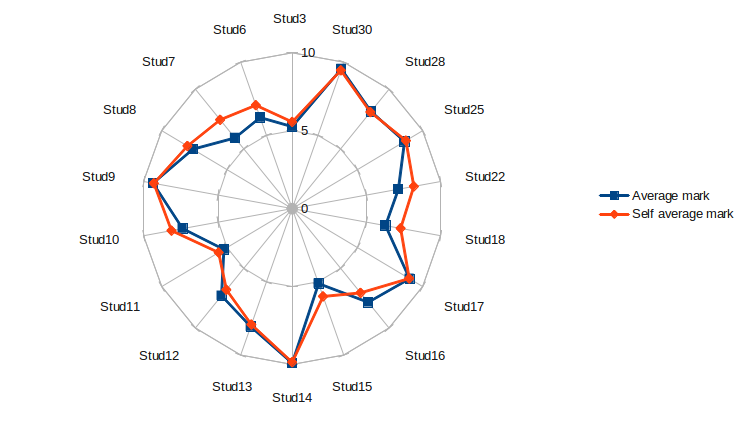
\includegraphics[width=12cm]{EvcWorkshop1.png}
	\caption{Grafo que muestra las diferentes calificaciones que se autoasignaron los estudiantes y la que les dieron sus compañeros.}
	\label{fig:EvcWorkshop1}
\end{figure}

Se puede decir que no hubo muchas diferencias en las calificaciones. Esto es un buen indicador, ya que la mayor parte de los estudiantes que tuvieron una diferencia grande en las primeras calificaciones, corrigieron esta desviación en las siguientes evaluaciones. Aunque también hay estudiantes que hicieron buenas auto-evaluaciones desde el principio, como se puede comprobar viendo la última columna de la tabla~\ref{tab:EvcWorkshop1}. En ella se representa la diferencia media de las calificaciones que recibieron y que se autoasignaron.

En este punto el profesor tuvo que decidir sobre la validez del indicador. Y en caso afirmativo, cuál seria el límite entre una valoración positiva y una negativa. Gracias a que el grupo era pequeño, el profesor podía comparar el comportamiento real observado durante el curso con los resultados del indicador, confirmando que había mucha similitud entre ambas calificaicones. De hecho, el límite positivo se estableció con una media de $0,5$ puntos o menos. Mientras que una valoración negativa se dejó para aquellos cuya diferencia era superior a $1$. Con estos resultados se obtuvo la siguiente distribución (provocando una distribución de campana).

\begin{itemize}
\item Si la diferencia media está entre $0$ y $0,5$, esto era un indicador positivo del desempeño de la competencia de la autocritica. (5 estudiantes).
\item Si la diferencia media está entre $0,5$ y $1$, los estudiantes mostraron un nivel medio de la competencia (9 estudiantes).
\item If the mean difference of the averages is $1$ or higher, esto era un indicador negativo del desempeño de la competencia de la autocritica (4 estudiantes).
\end{itemize}

Por supuesto, se necesitan más estudios para determinar la validez de los resultados de EvalCourse como indicadores de la competencia. Sin embargo, en nuestro caso, pudimos decir que la informaicón fue de utilidad para justificar la evaluación de los estudiantes.

\subsection{Resultados}

Morbi at augue sapien. Duis tempus quam vitae velit interdum ultricies. Vivamus laoreet lacinia elit sit amet vehicula. Ut congue diam ac magna hendrerit sed fermentum justo lacinia. Curabitur vel odio neque, quis consequat mi. Proin lobortis justo quis enim fermentum accumsan sagittis ipsum imperdiet. Proin sem felis, laoreet placerat egestas id, fringilla id mauris. Pellentesque a nisi sit amet leo consectetur gravida nec et dui. Curabitur quis hendrerit augue. Etiam sed dui nec tortor convallis fringilla. Proin tempor mattis diam nec egestas. Quisque condimentum elementum lacus ac porta.

% EVALSIM ---------------------------------------------------------------------------------
\section{EvalSim aplicado a los mundos virtuales}

Morbi at augue sapien. Duis tempus quam vitae velit interdum ultricies. Vivamus laoreet lacinia elit sit amet vehicula. Ut congue diam ac magna hendrerit sed fermentum justo lacinia. Curabitur vel odio neque, quis consequat mi. Proin lobortis justo quis enim fermentum accumsan sagittis ipsum imperdiet. Proin sem felis, laoreet placerat egestas id, fringilla id mauris. Pellentesque a nisi sit amet leo consectetur gravida nec et dui. Curabitur quis hendrerit augue. Etiam sed dui nec tortor convallis fringilla. Proin tempor mattis diam nec egestas. Quisque condimentum elementum lacus ac porta. Vivamus congue, odio eu ullamcorper elementum, leo turpis tempus sem, at condimentum dolor quam eu nunc. Pellentesque eget risus ac velit aliquam sollicitudin sed et ipsum. 

\section{Evaluación}

Morbi at augue sapien. Duis tempus quam vitae velit interdum ultricies. Vivamus laoreet lacinia elit sit amet vehicula. Ut congue diam ac magna hendrerit sed fermentum justo lacinia. Curabitur vel odio neque, quis consequat mi. Proin lobortis justo quis enim fermentum accumsan sagittis ipsum imperdiet. Proin sem felis, laoreet placerat egestas id, fringilla id mauris. Pellentesque a nisi sit amet leo consectetur gravida nec et dui. Curabitur quis hendrerit augue. Etiam sed dui nec tortor convallis fringilla. Proin tempor mattis diam nec egestas. Quisque condimentum elementum lacus ac porta. Vivamus congue, odio eu ullamcorper elementum, leo turpis tempus sem, at condimentum dolor quam eu nunc. Pellentesque eget risus ac velit aliquam sollicitudin sed et ipsum. 

\section{Conclusiones}

Morbi at augue sapien. Duis tempus quam vitae velit interdum ultricies. Vivamus laoreet lacinia elit sit amet vehicula. Ut congue diam ac magna hendrerit sed fermentum justo lacinia. Curabitur vel odio neque, quis consequat mi. Proin lobortis justo quis enim fermentum accumsan sagittis ipsum imperdiet. Proin sem felis, laoreet placerat egestas id, fringilla id mauris. Pellentesque a nisi sit amet leo consectetur gravida nec et dui. Curabitur quis hendrerit augue. Etiam sed dui nec tortor convallis fringilla. Proin tempor mattis diam nec egestas. Quisque condimentum elementum lacus ac porta. Vivamus congue, odio eu ullamcorper elementum, leo turpis tempus sem, at condimentum dolor quam eu nunc. Pellentesque eget risus ac velit aliquam sollicitudin sed et ipsum. 








% ----------------------------------------------------------------------

